A continuacion se establecerá como fueron ejecutadas las mediciones del circuito construido. Los esquemas se elaboraron en proteus y son representativos, se debe hacer caso omiso a la nomenclatura de estos. Es importante mencionar que el generador de señales es representado en los esquematicos como una fuente de tension AC.

\subsection{Setup General}
A continuación se vera un acercamiento a las formas de las mediciones a nivel general, las conexiones utilizadas y el espacio de trabajo.

\begin{figure}[H]
    \centering
    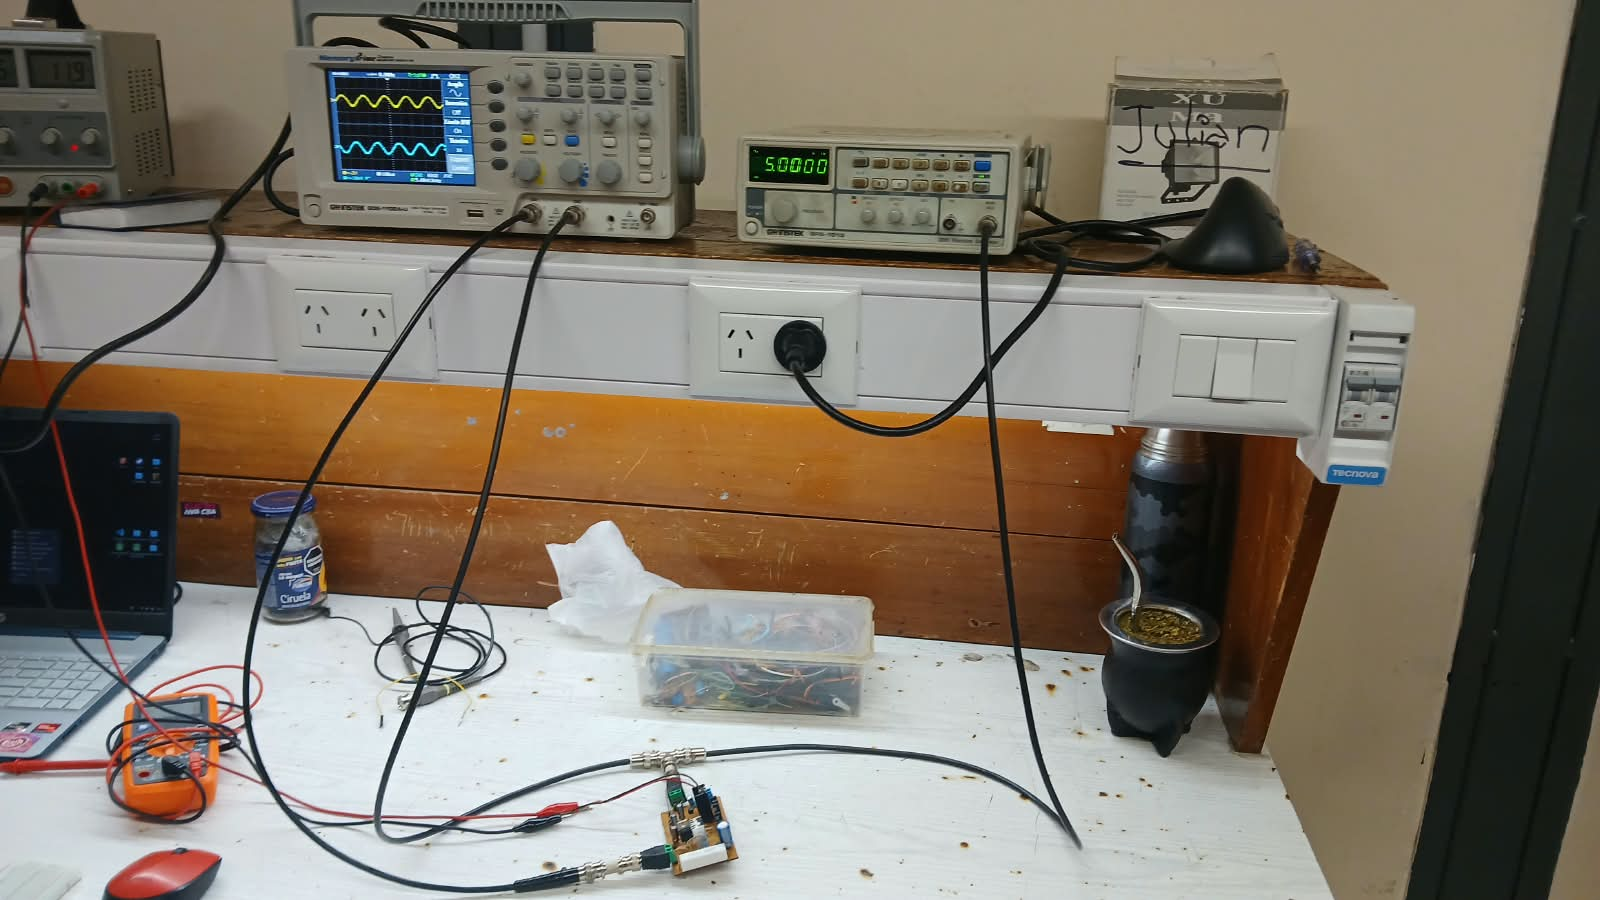
\includegraphics[width=0.8\textwidth]{FotosMed/Setup/SetupGeneral1.jpeg}
    \caption{Distribucion General}
    \label{fig:DistribucionGeneral}
\end{figure}

\begin{figure}[H]
    \centering
    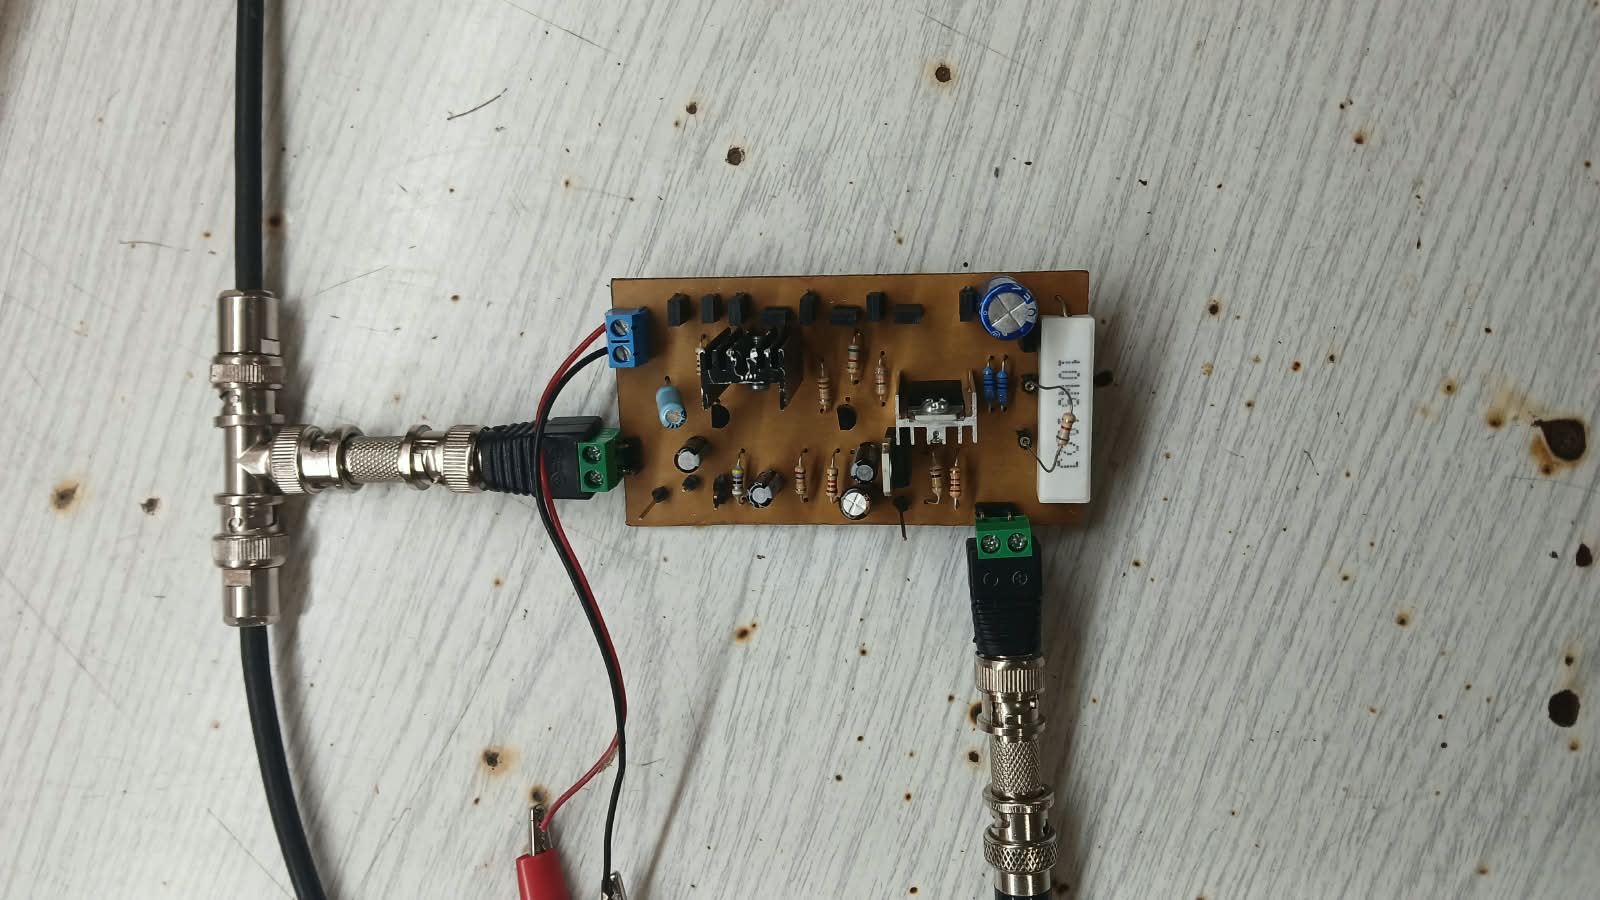
\includegraphics[width=0.8\textwidth]{FotosMed/Setup/PlacaConectada.jpeg}
    \caption{Conexion a Placa}
    \label{fig:placa}
\end{figure}

\begin{figure}[H]
    \centering
    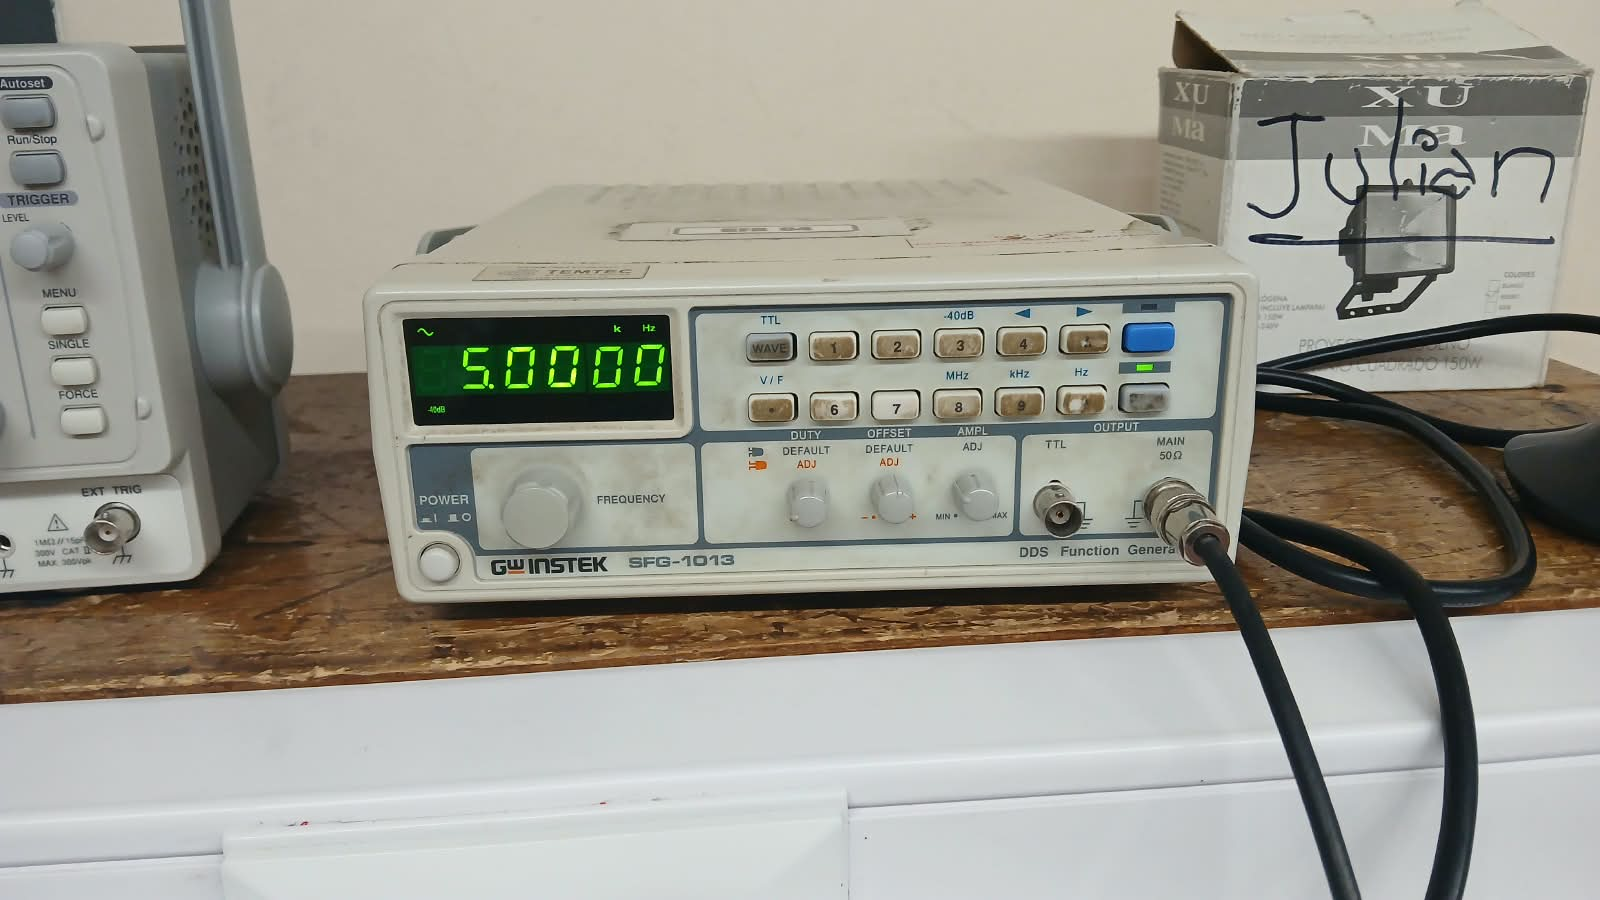
\includegraphics[width=0.8\textwidth]{FotosMed/Setup/Generador.jpeg}
    \caption{Generador}
    \label{fig:GeneradorGeneral}
\end{figure}

\begin{figure}[H]
    \centering
    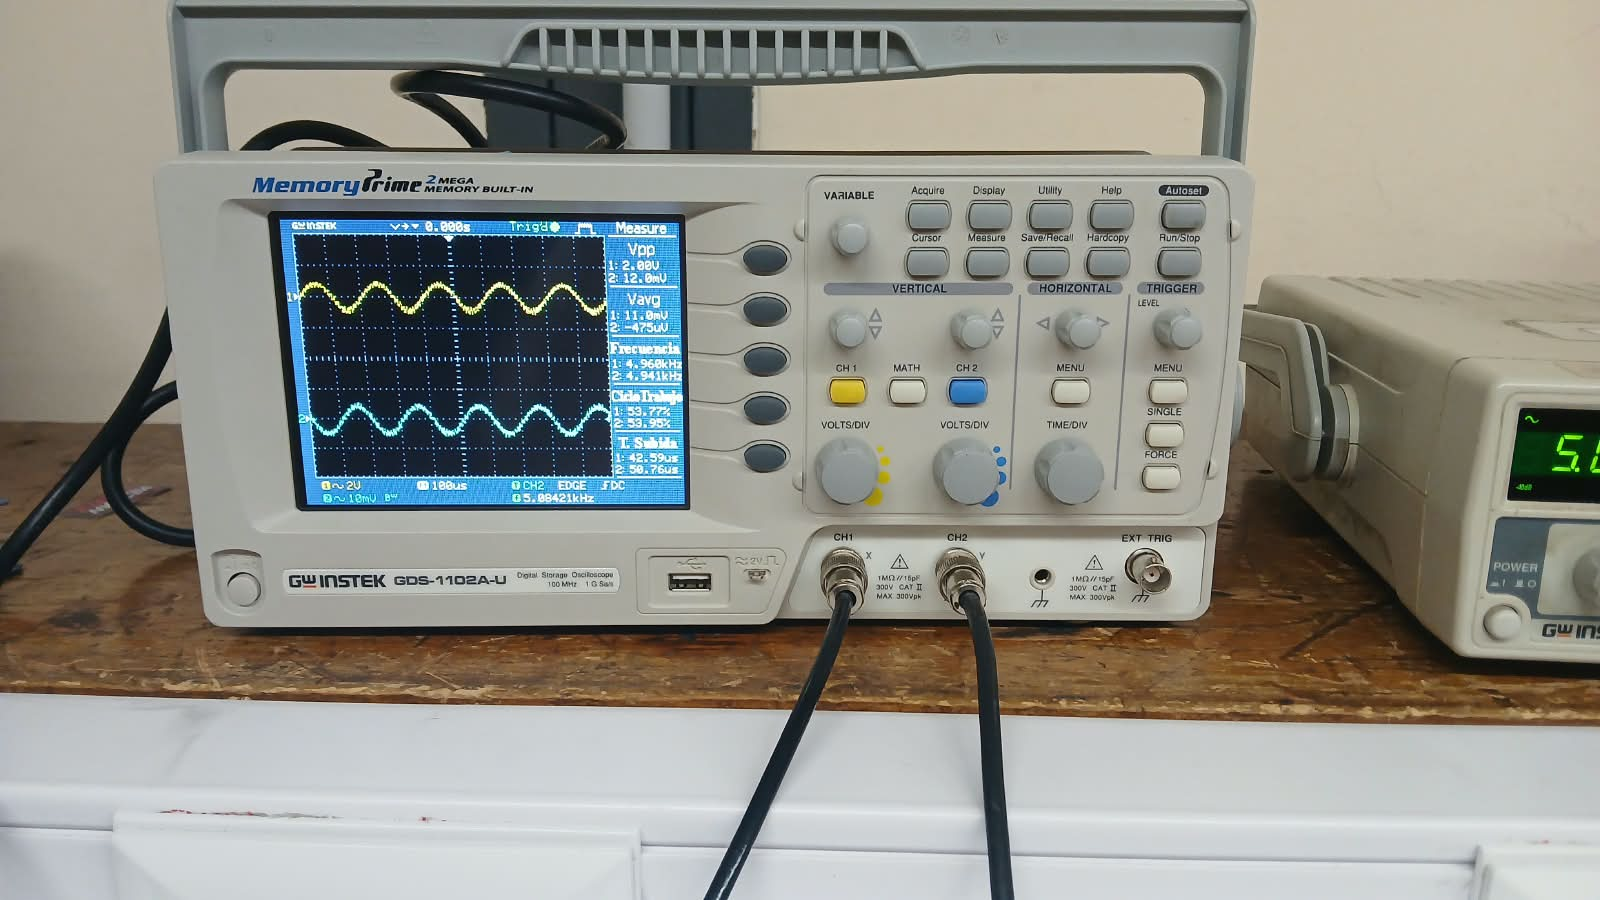
\includegraphics[width=0.8\textwidth]{FotosMed/Setup/Osc.jpeg}
    \caption{Osciloscopio}
    \label{fig:OscGeneral}
\end{figure}


\subsection{Medicion de Transistores}
Realizadas con el multímetro de trabajo, se evaluaron la caída de tensión de cada uno de los componentes teniendo precauciones de evitar el contacto entre terminales. Se aprovecharon los jumpers incluidos en el disenio para realizar las mediciones de corriente de colector de los transistores.

\begin{figure}[H]
    \centering
    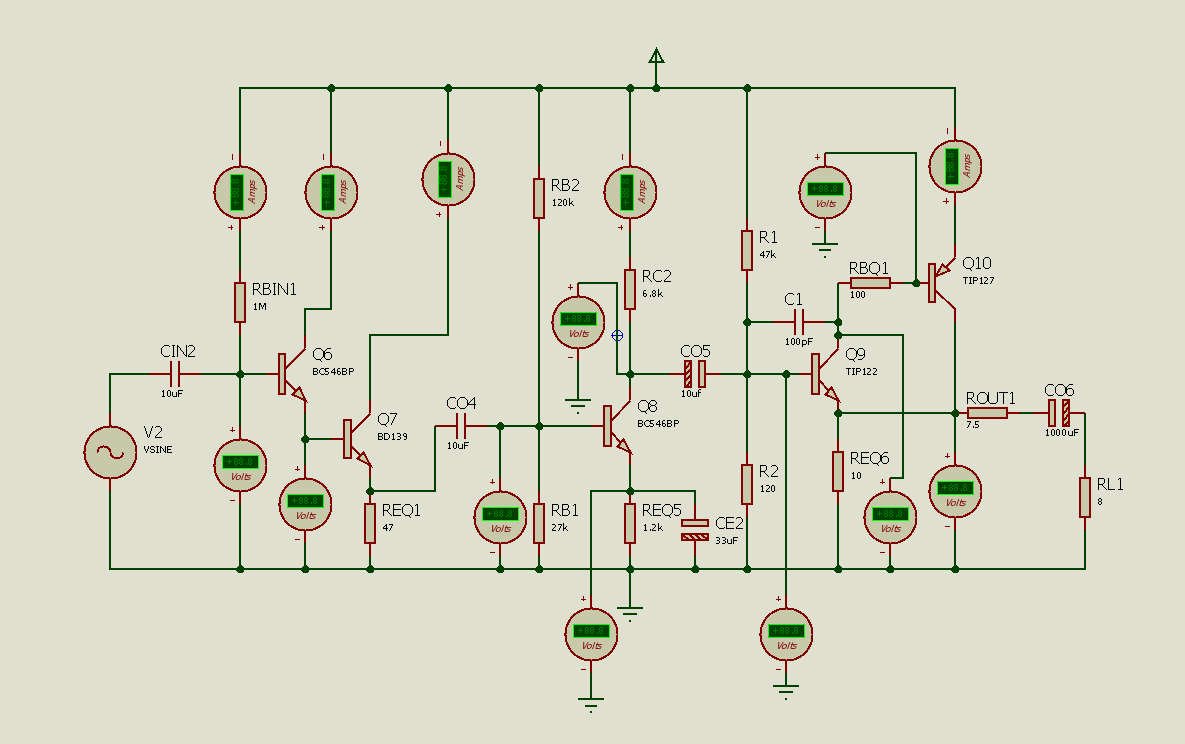
\includegraphics[width=0.8\textwidth]{SetupMediciones/TensionesCorrientes/VITransistores.png}
    \caption{Esquema de Medición de Transistores}
    \label{fig:esquematicoTransistores}
\end{figure}

Como se puede observar en la Figura \ref{fig:esquematicoTransistores}, estas mediciones de tension y corriente fueron exclusivamente realizadas para el calculo de potencia de los transistores, se debe remarcar aqui que la corriente de colector del transistor NPN del Sziklai fue hecha de manera indirecta, midiendo la caida de tension en la resistencia de base del pnp.

\begin{figure}[H]
    \centering
    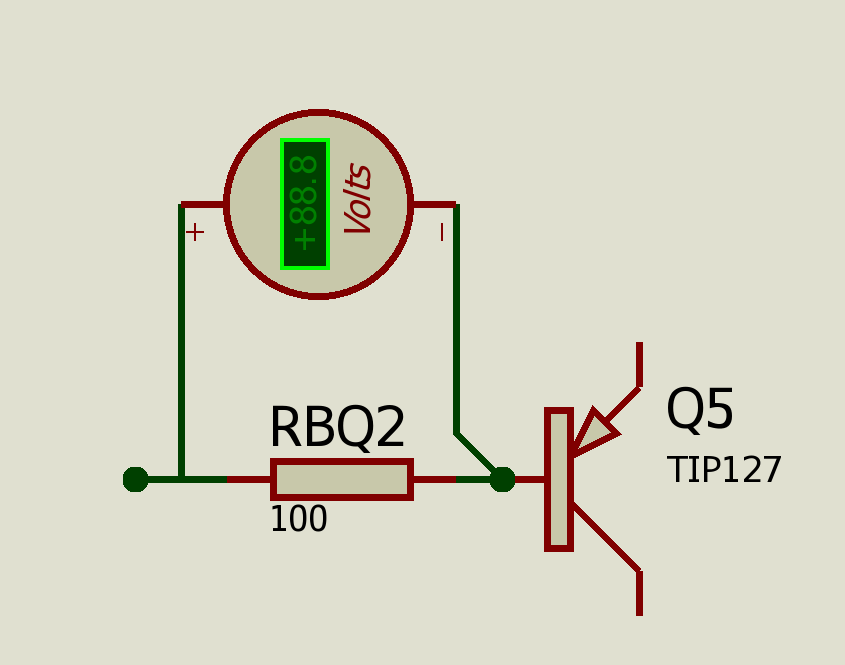
\includegraphics[width=0.8\textwidth]{SetupMediciones/TensionesCorrientes/IcQ4.png}
    \caption{Medición Indirecta}
    \label{fig:esquematicoICQ4}
\end{figure}

Como se puede observar en la Figura \ref{fig:esquematicoICQ4}, una vez medida la tension de la resistencia, se obtuvo Ic para los cálculos de potencia.

\subsection{Medición de Resistencias}
Similar al caso anterior, estas también fueron ejecutadas mediante un multímetro digital.

\begin{figure}[H]
    \centering
    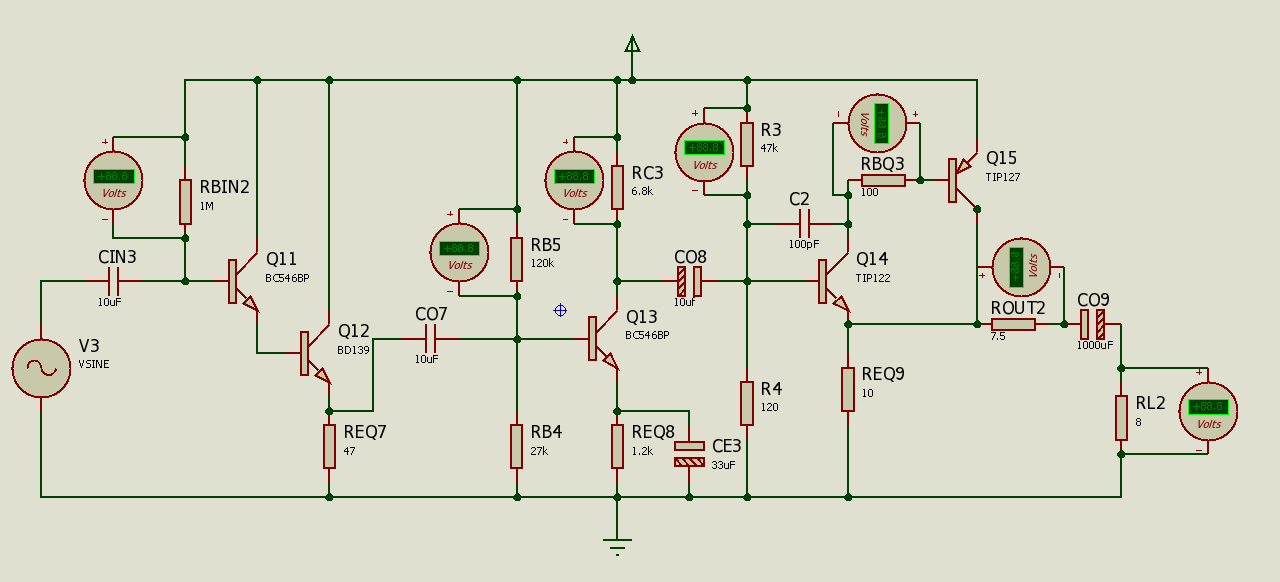
\includegraphics[width=0.8\textwidth]{SetupMediciones/TensionesCorrientes/VResitecnias.png}
    \caption{Esquema de Medición de Resistencias}
    \label{fig:esquematicoResistencias}
\end{figure}

Una vez obtenidas las mediciones de la Figura \ref{fig:esquematicoResistencias}, se determino la potencia disipada mediante la Ley de Ohm.

\subsection{Barrido de Amplitud}
Esta medición es realizada en 3 configuraciones:
    - Darlington
    - Darlinton y Emisor Comun
    - Circuito completo

En esta, las amplitudes de entrada a las configuraciones irán aumentando, esto se realizo incrementando la amplitud de salida del generador de señales.

\subsubsection{Barrido de Etapa 1}
A conitunuacion se presenta el esquema y foto del método de medicion utilizado en la etapa 1(Darlington).

\begin{figure}[H]
    \centering
    % Primera minipage (ocupa el 45% del ancho de la página)
    \begin{minipage}{0.45\textwidth}
        \centering
        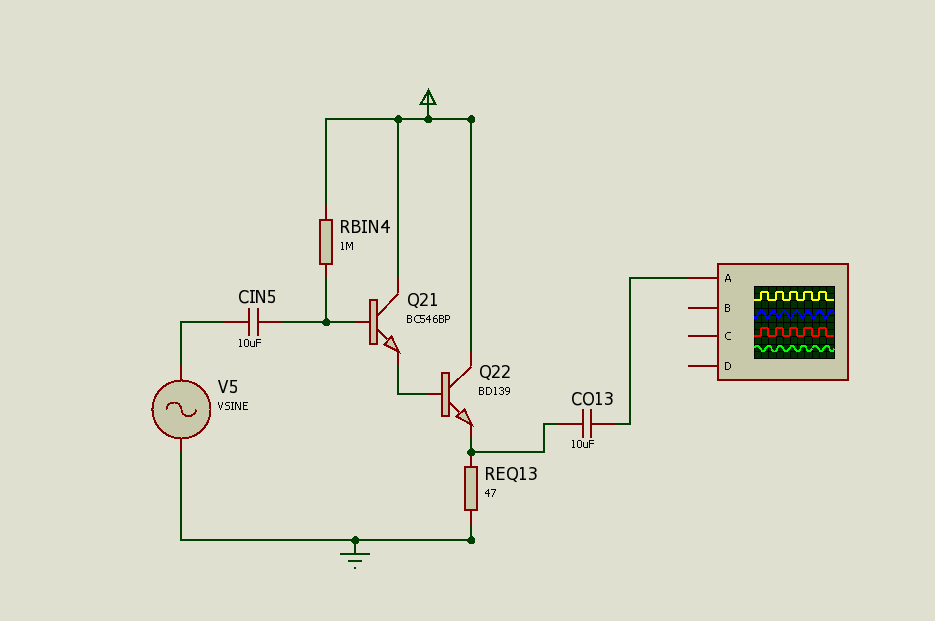
\includegraphics[width=\textwidth]{SetupMediciones/TensionesCorrientes/VMaxMinDAR.png} % Ajusta el ancho al de la minipage
        \caption{Representacion esquematica.}
        \label{fig:esquematicpBarridoEtapa1}
    \end{minipage}
    \hfill % Relleno elástico para separar las imágenes
    % Segunda minipage (ocupa el 45% del ancho de la página)
    \begin{minipage}{0.45\textwidth}
        \centering        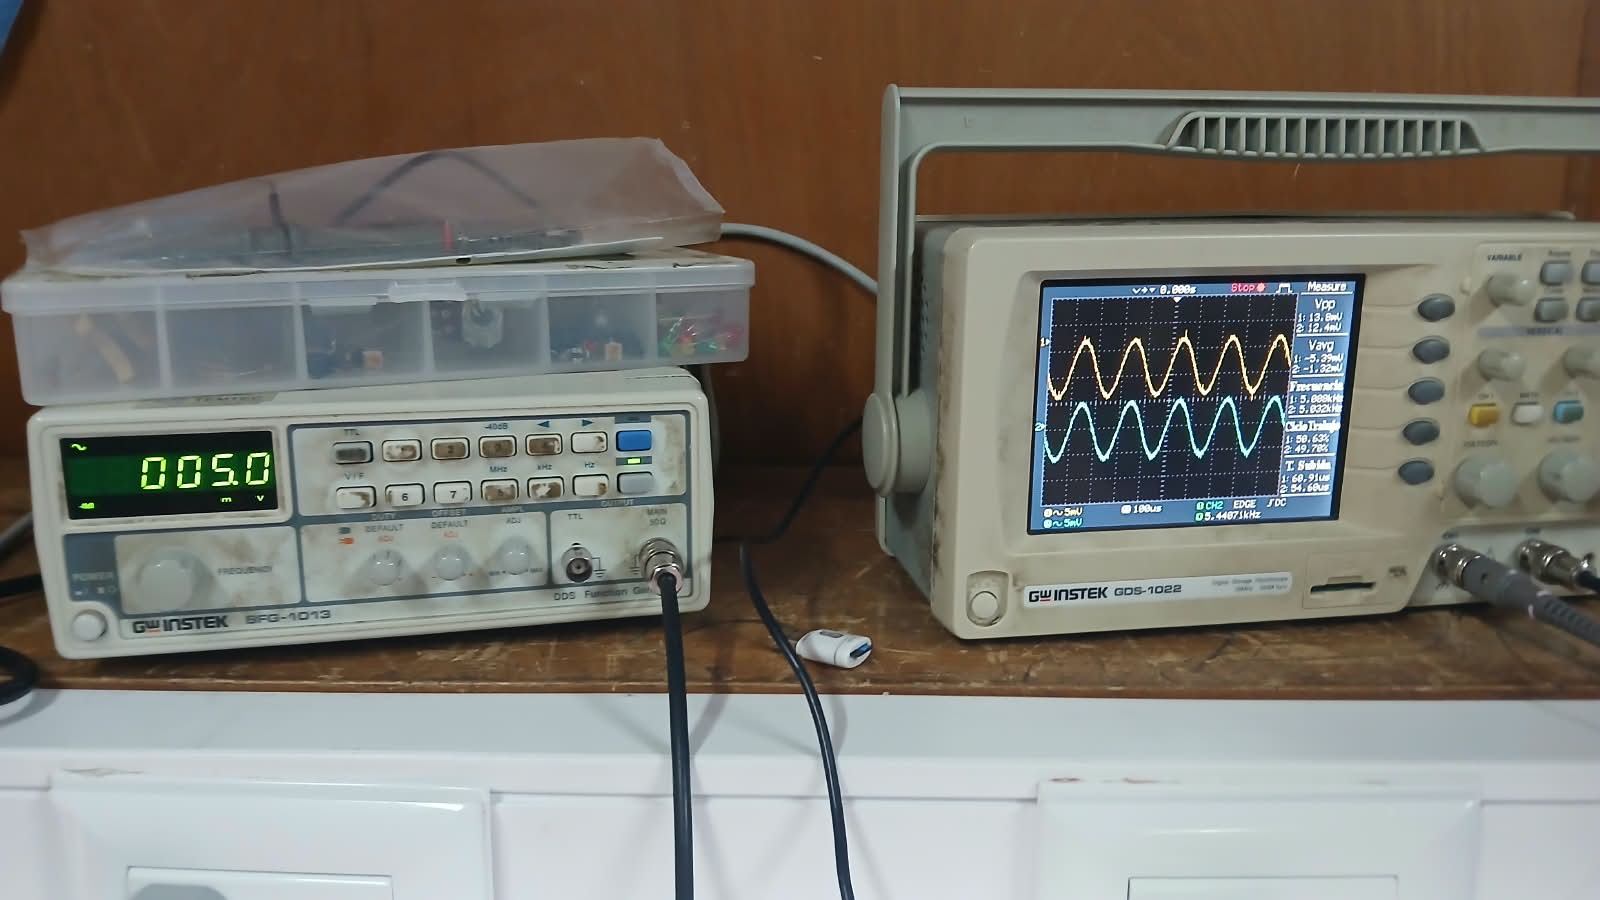
\includegraphics[width=\textwidth]{FotosMed/Barrido de amplitud/E1/5m.jpeg}
        \caption{Imagen de la Medicion.}
        \label{fig:medicionBarridoEtapa1}
    \end{minipage}
\end{figure}

\begin{figure}[H]
    \centering
    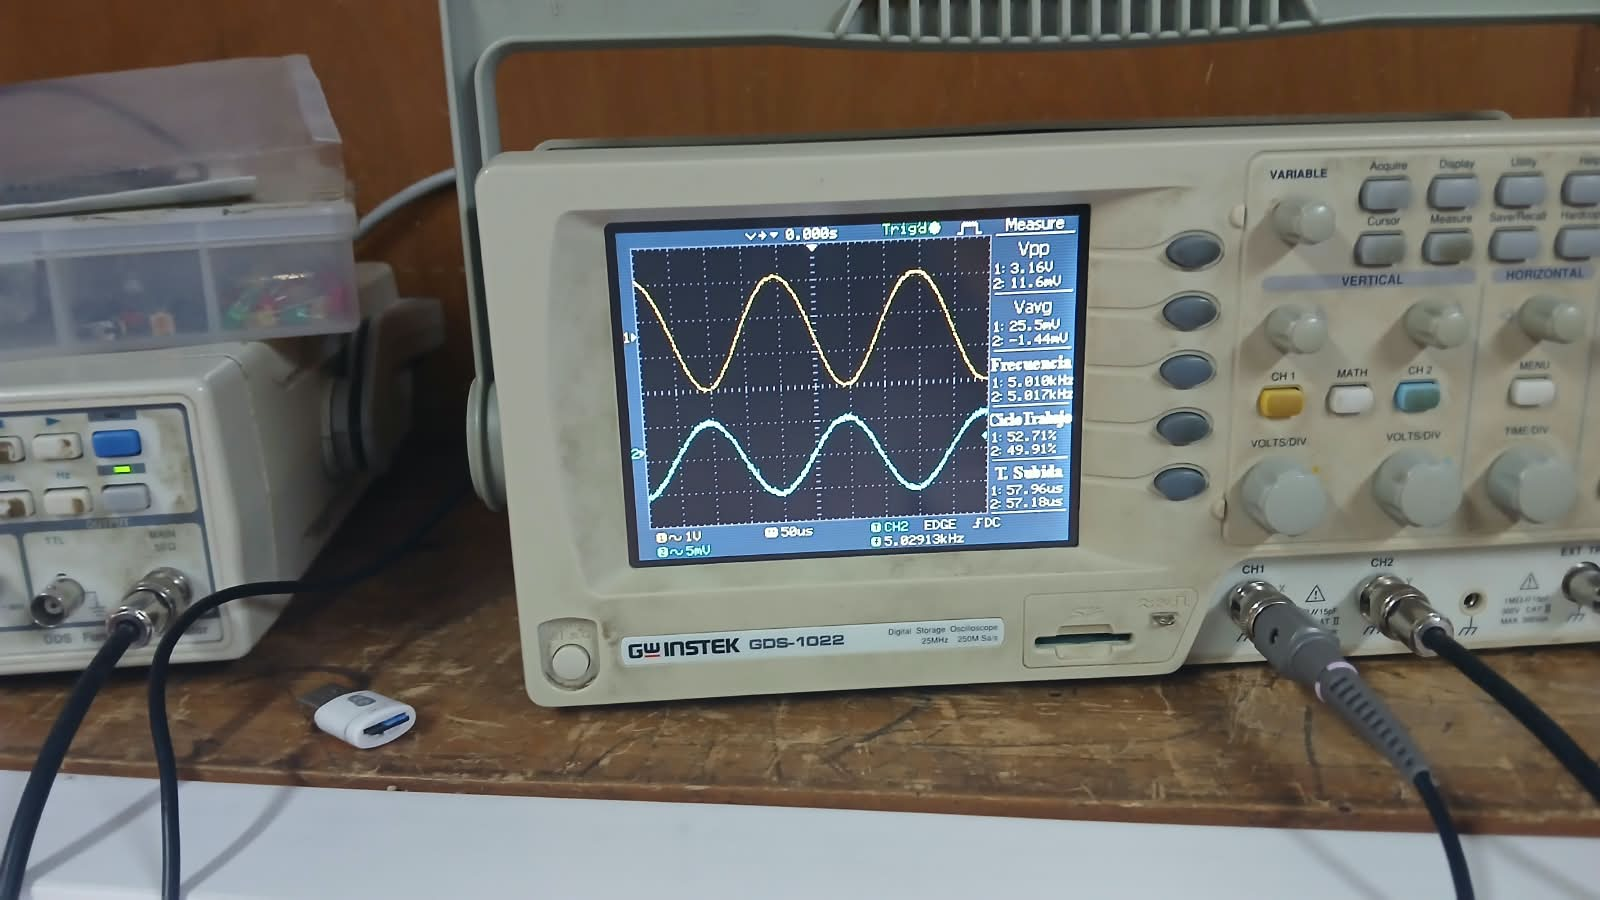
\includegraphics[width=0.8\textwidth]{FotosMed/Barrido de amplitud/E12/5mzoom.jpeg}
    \caption{Pantalla del Osciloscopio}
    \label{fig:osciloscopioBarridoEtapa1}
\end{figure}

Se puede ver en \ref{fig:osciloscopioBarridoEtapa1}, la tension de entrada esta en el canal 1 del osciloscopio (estipulada a 13.8 mV pico a pico) mientras que la salida se observa en el canal 2.

\subsubsection{Barrido de Etapa 1 y 2}
Semejante al anterior, la tensión de entrada sigue siendo variada incrementando el dial del generador en modo amplitud, con la leve diferencia de que esta configuración esta constituida por las etapas 1 y 2 en conjunto.

\begin{figure}[H]
    \centering
    % Primera minipage (ocupa el 45% del ancho de la página)
    \begin{minipage}{0.45\textwidth}
        \centering
        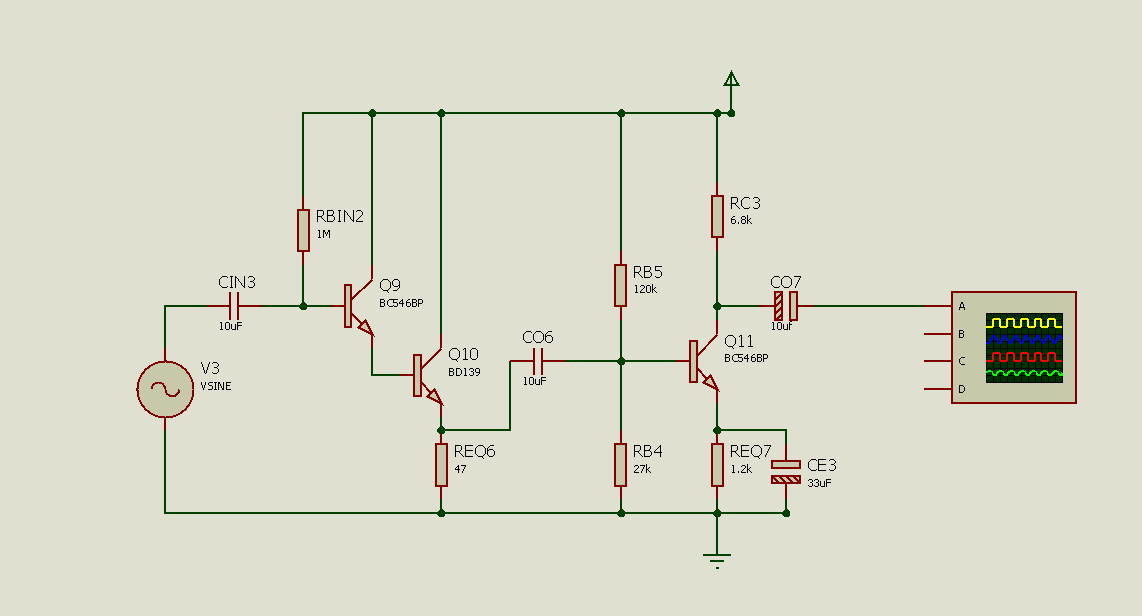
\includegraphics[width=\textwidth]{SetupMediciones/ZOUT/Zout12VACIO.png} % Ajusta el ancho al de la minipage
        \caption{Representacion esquematica.}
        \label{fig:esquematicpBar12}
    \end{minipage}
    \hfill % Relleno elástico para separar las imágenes
    % Segunda minipage (ocupa el 45% del ancho de la página)
    \begin{minipage}{0.45\textwidth}
        \centering
        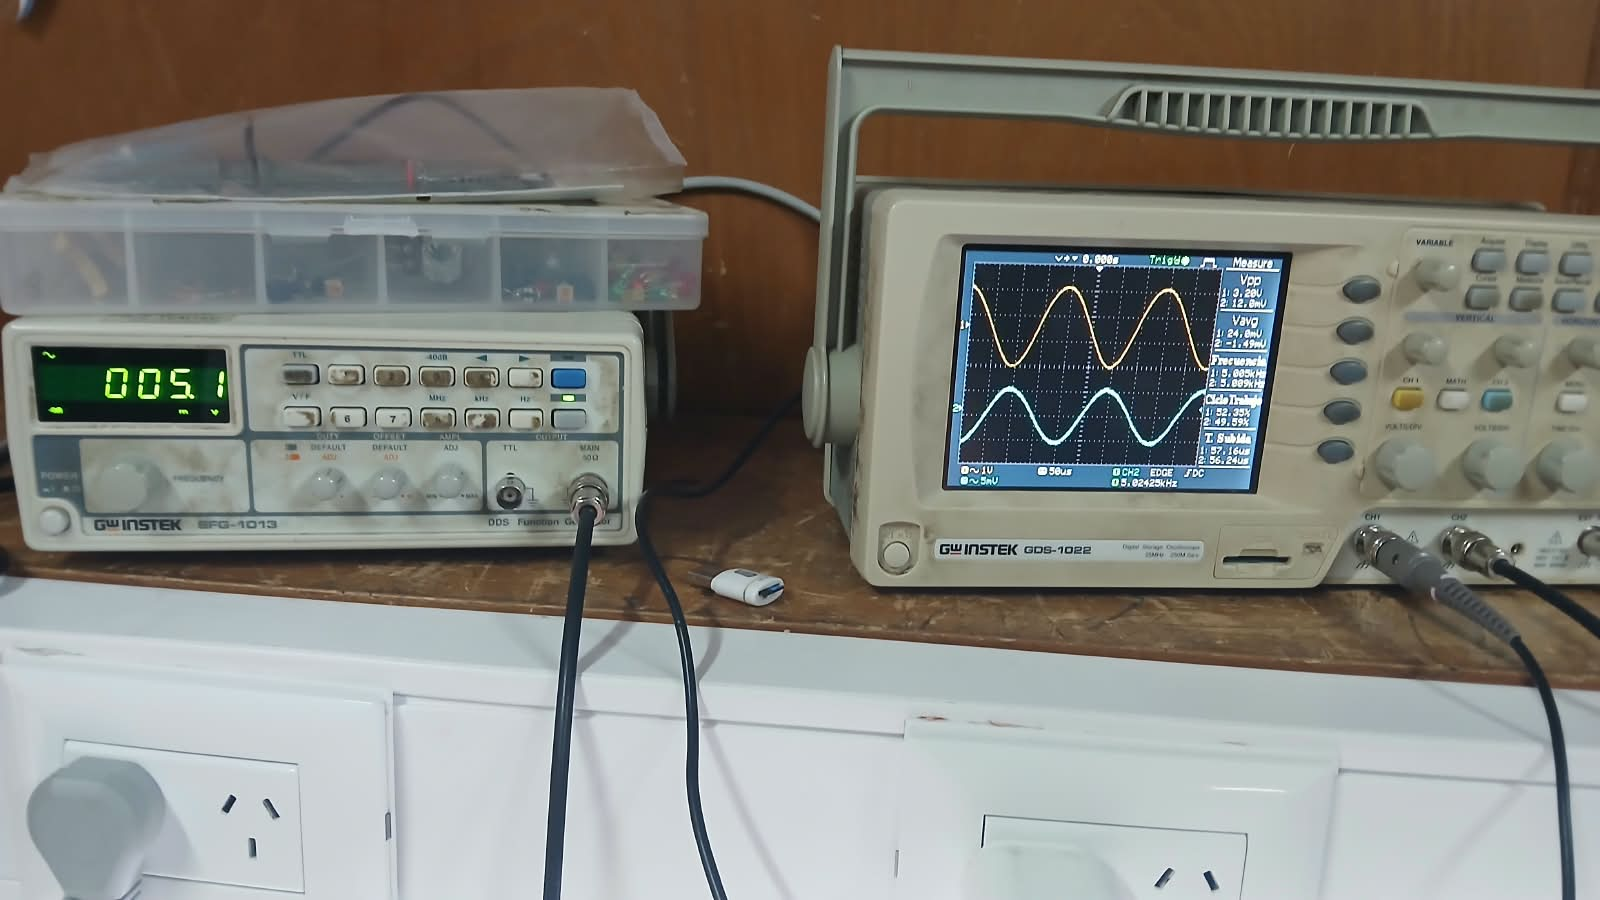
\includegraphics[width=\textwidth]{FotosMed/Barrido de amplitud/E12/5m.jpeg}
        \caption{Imagen de la Medicion.}
        \label{fig:medicionbar12}
    \end{minipage}
\end{figure}

\begin{figure}[H]
    \centering
    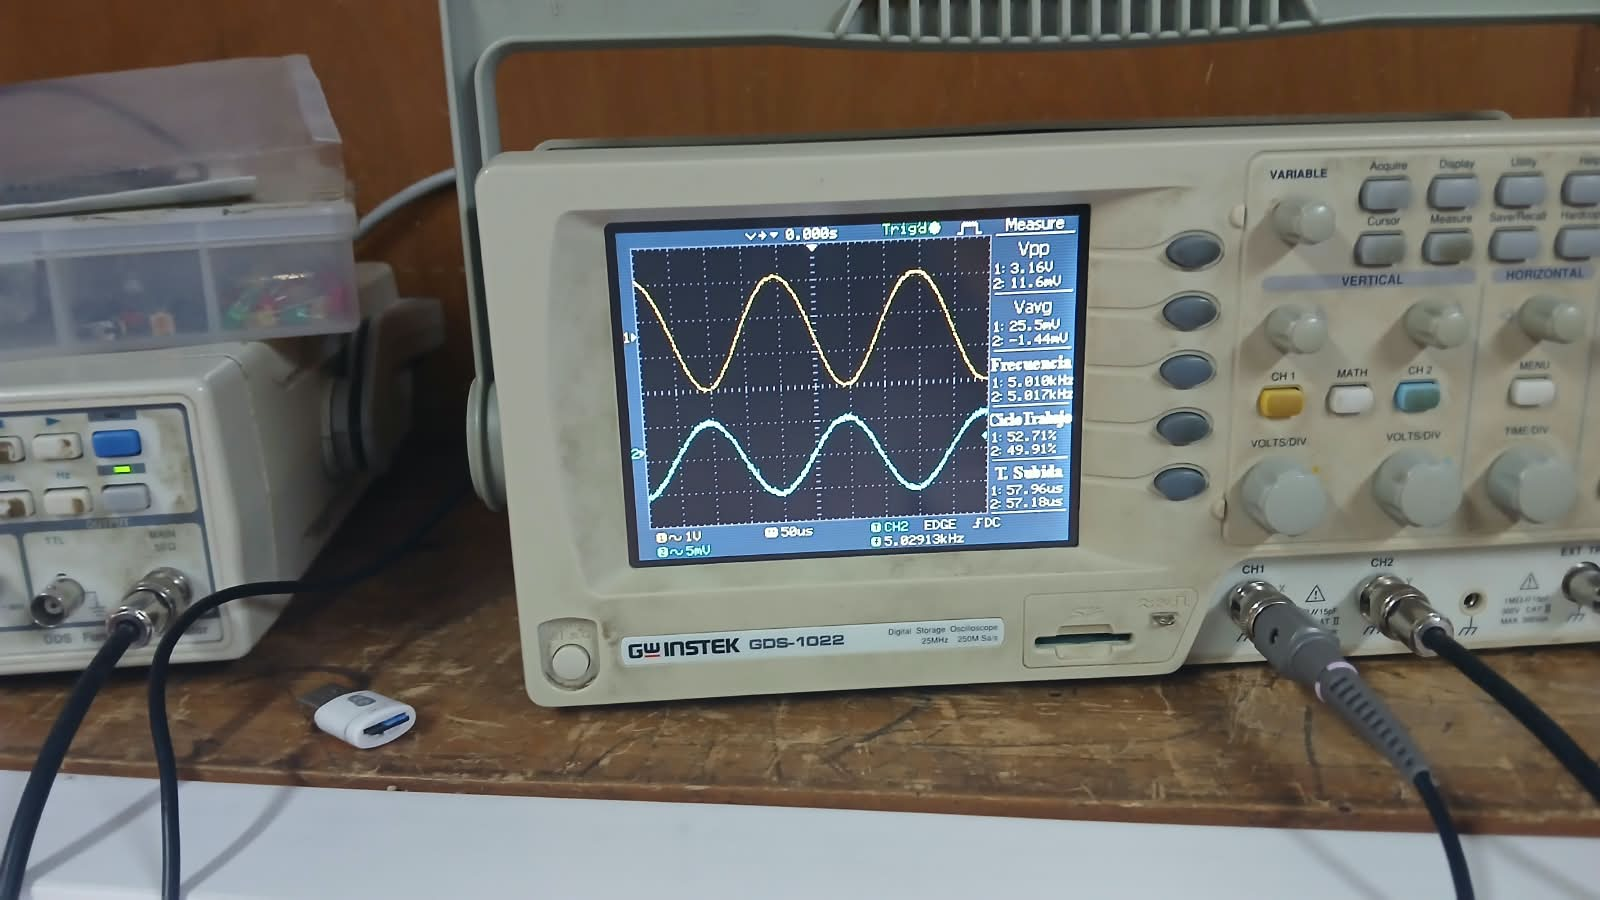
\includegraphics[width=0.8\textwidth]{FotosMed/Barrido de amplitud/E12/5mzoom.jpeg}
    \caption{Pantalla del Osciloscopio}
    \label{fig:osciloscopioBArr12}
\end{figure}

Se puede ver en \ref{fig:osciloscopioBArr12} la tension de entrada esta en el canal 2 del osciloscopio mientras que la salida se observa en el canal 1.

\subsection{Barrido del circuito completo}
Su unica distinción es que esta es realizada sin necesidad de modificar el circuito, se mide desde la entrada hasta la ultima etapa

\begin{figure}[H]
    \centering
    % Primera minipage (ocupa el 45% del ancho de la página)
    \begin{minipage}{0.45\textwidth}
        \centering
        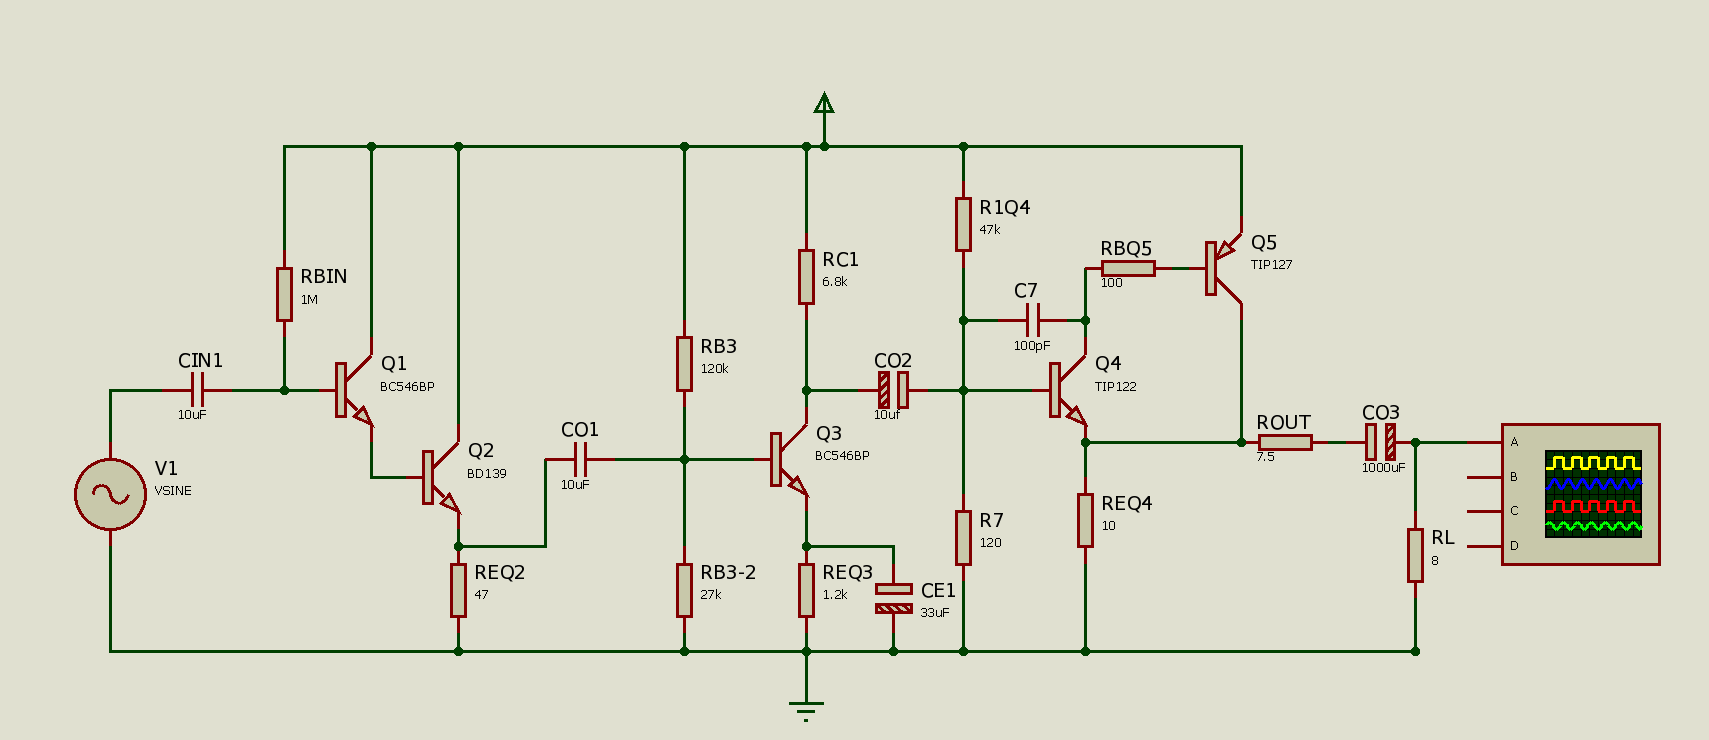
\includegraphics[width=\textwidth]{SetupMediciones/TensionesCorrientes/BarridoDeFrecuencia.png} % Ajusta el ancho al de la minipage
        \caption{Representacion esquematica.}
        \label{fig:esquematicoBarCompleto}
    \end{minipage}
    \hfill % Relleno elástico para separar las imágenes
    % Segunda minipage (ocupa el 45% del ancho de la página)
    \begin{minipage}{0.45\textwidth}
        \centering
        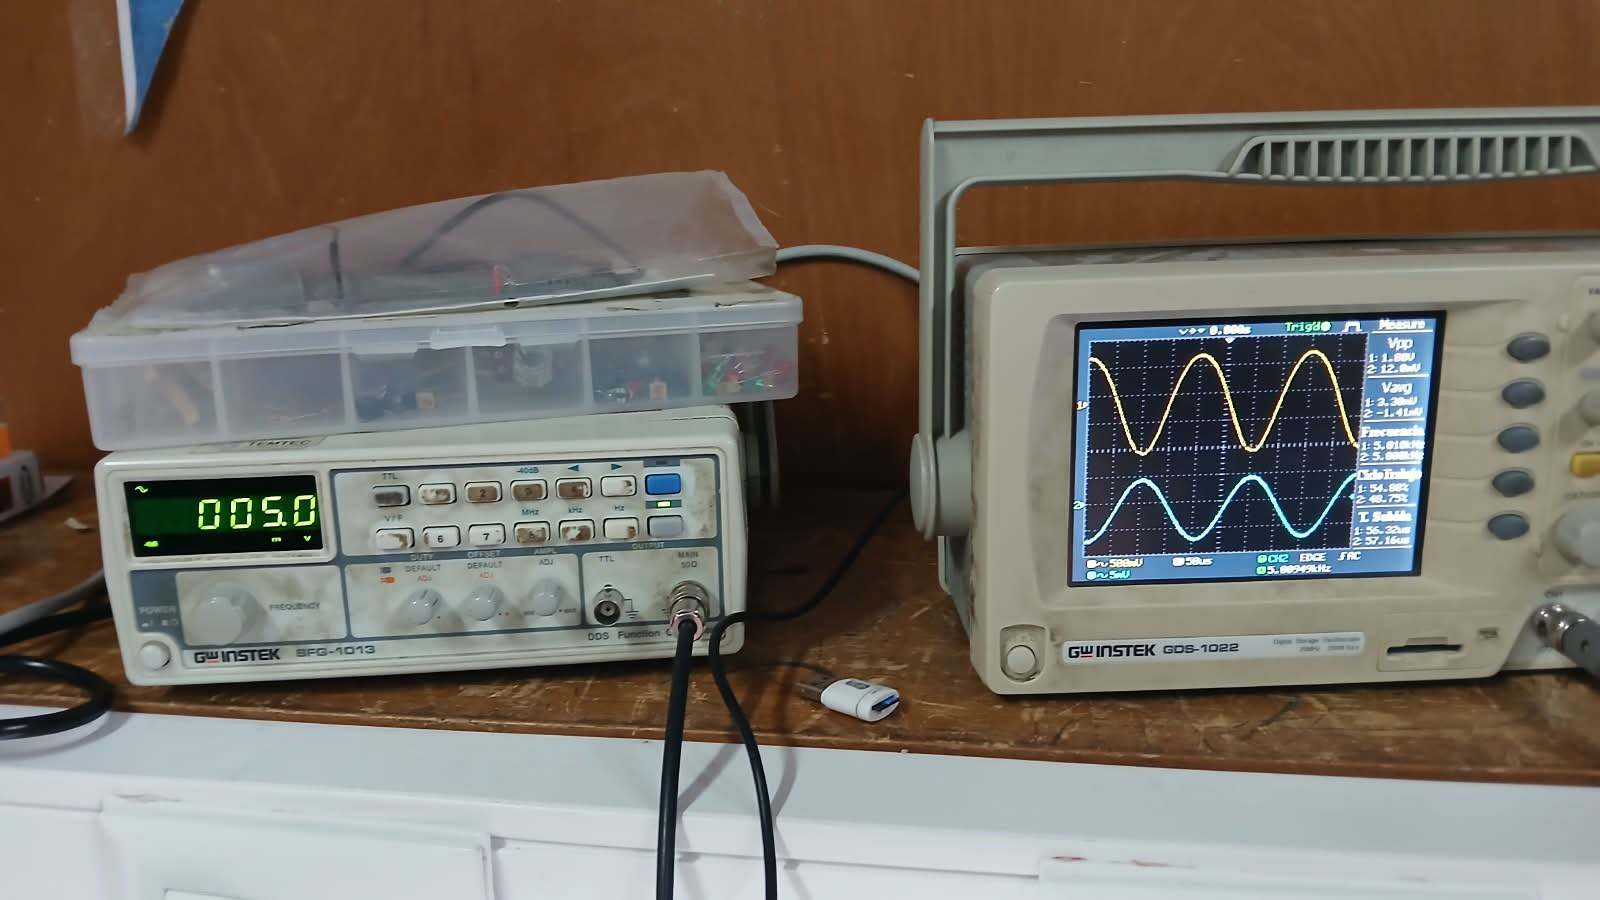
\includegraphics[width=\textwidth]{FotosMed/Barrido de amplitud/ETOTAL/5m.jpeg}
        \caption{Imagen de la Medición.}
        \label{fig:medicionBArCompleto}
    \end{minipage}
\end{figure}

\begin{figure}[H]
    \centering
    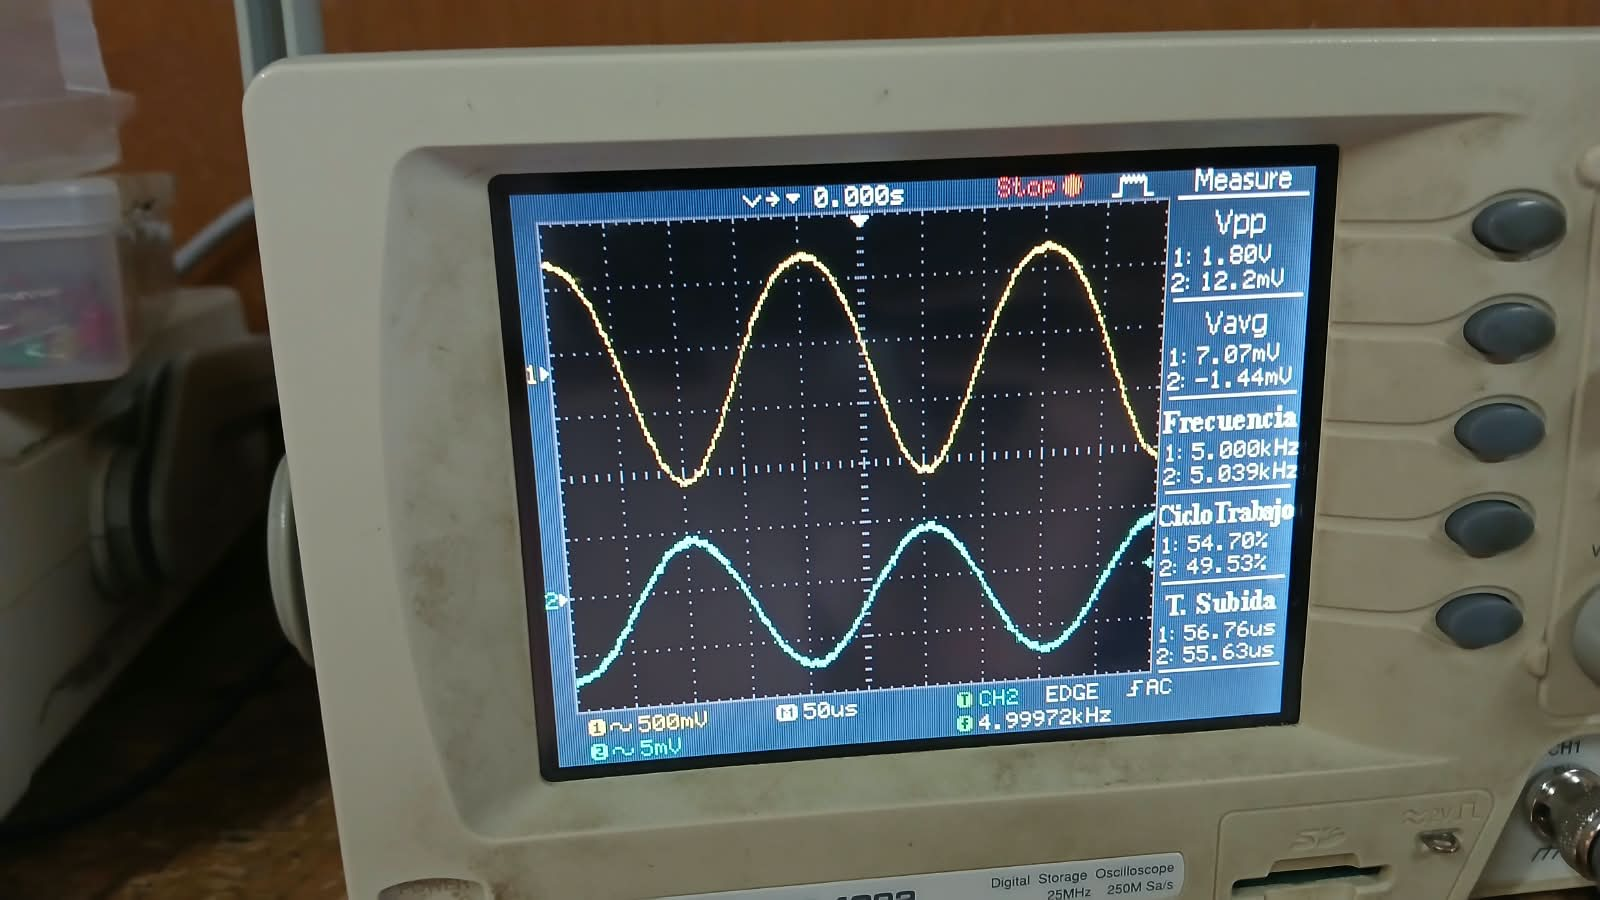
\includegraphics[width=0.8\textwidth]{FotosMed/Barrido de amplitud/ETOTAL/5mzoom.jpeg}
    \caption{Pantalla del Osciloscopio}
    \label{fig:osciloscopioBarCompleto}
\end{figure}

Se puede ver en \ref{fig:osciloscopioBarCompleto}, la tension de entrada esta en el canal 2 del osciloscopio(estipulada a 13.8 mV pico a pico) mientras que la salida se observa en el canal 1.

\subsection{Barrido de Frecuencia}
Realizada puramente observando el osciloscopio, se fue variando la frecuencia de salida del generador de decada en decada a medida que se realizaaban los calculos de ganancia, la amplitud de entrada fue establecida en 5,1 mV pico a pico.

Estas fueron realizadas en 3 configuraciones:
- Etapa 1 (Darlington)
- Etapa 1 y 2
- Circuito Completo

\subsubsection{Barrido de Etapa 1}
Utilizando la punta compensada conectada al osciloscopio se evaluó la tensión de salida de la primer etapa y se realizo el calculo de ganancia.

\begin{figure}[H]
    \centering
    % Primera minipage (ocupa el 45% del ancho de la página)
    \begin{minipage}{0.45\textwidth}
        \centering
        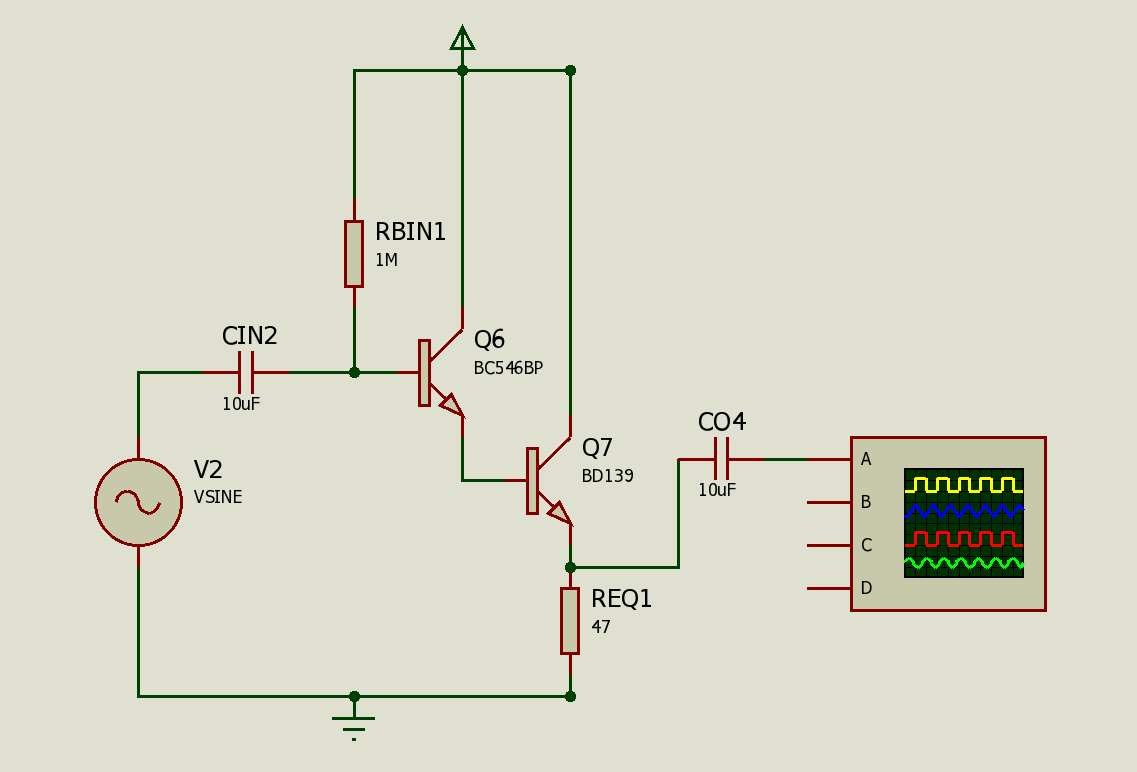
\includegraphics[width=\textwidth]{SetupMediciones/ZOUT/ZoutDARSinCarga.png} % Ajusta el ancho al de la minipage
        \caption{Representacion esquematica.}
        \label{fig:esquematicoBarFrec}
    \end{minipage}
    \hfill % Relleno elástico para separar las imágenes
    % Segunda minipage (ocupa el 45% del ancho de la página)
    \begin{minipage}{0.45\textwidth}
        \centering
        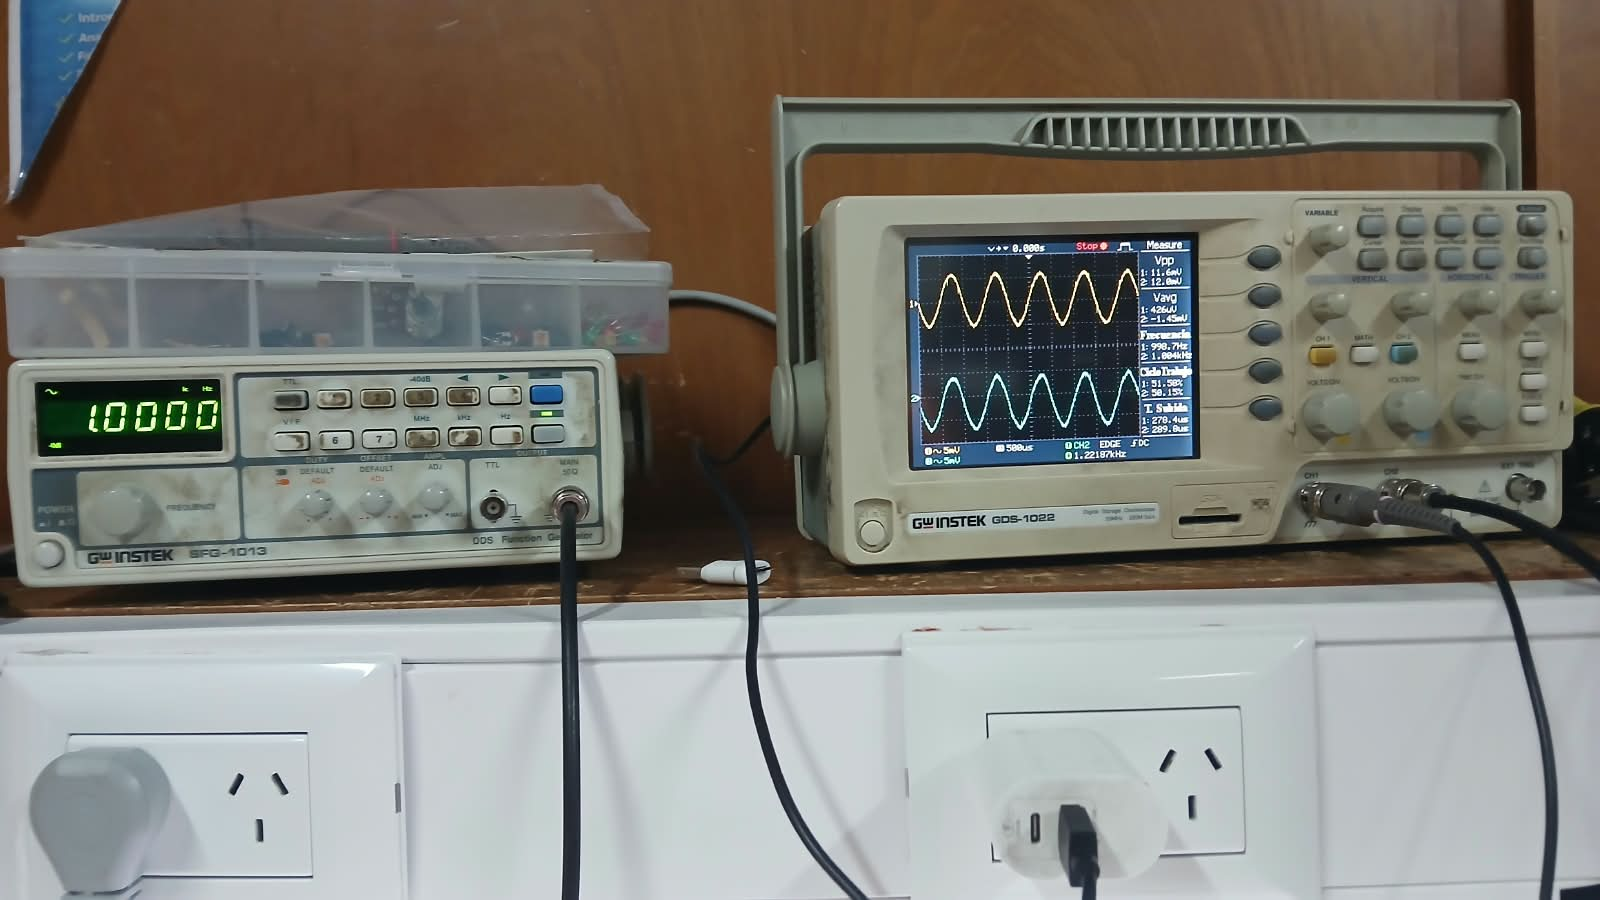
\includegraphics[width=\textwidth]{FotosMed/Barrido de frecuencia/E1/1k.jpeg}
        \caption{Imagen de la Medicion.}
        \label{fig:medicionBarFrec}
    \end{minipage}
\end{figure}

\begin{figure}[H]
    \centering
    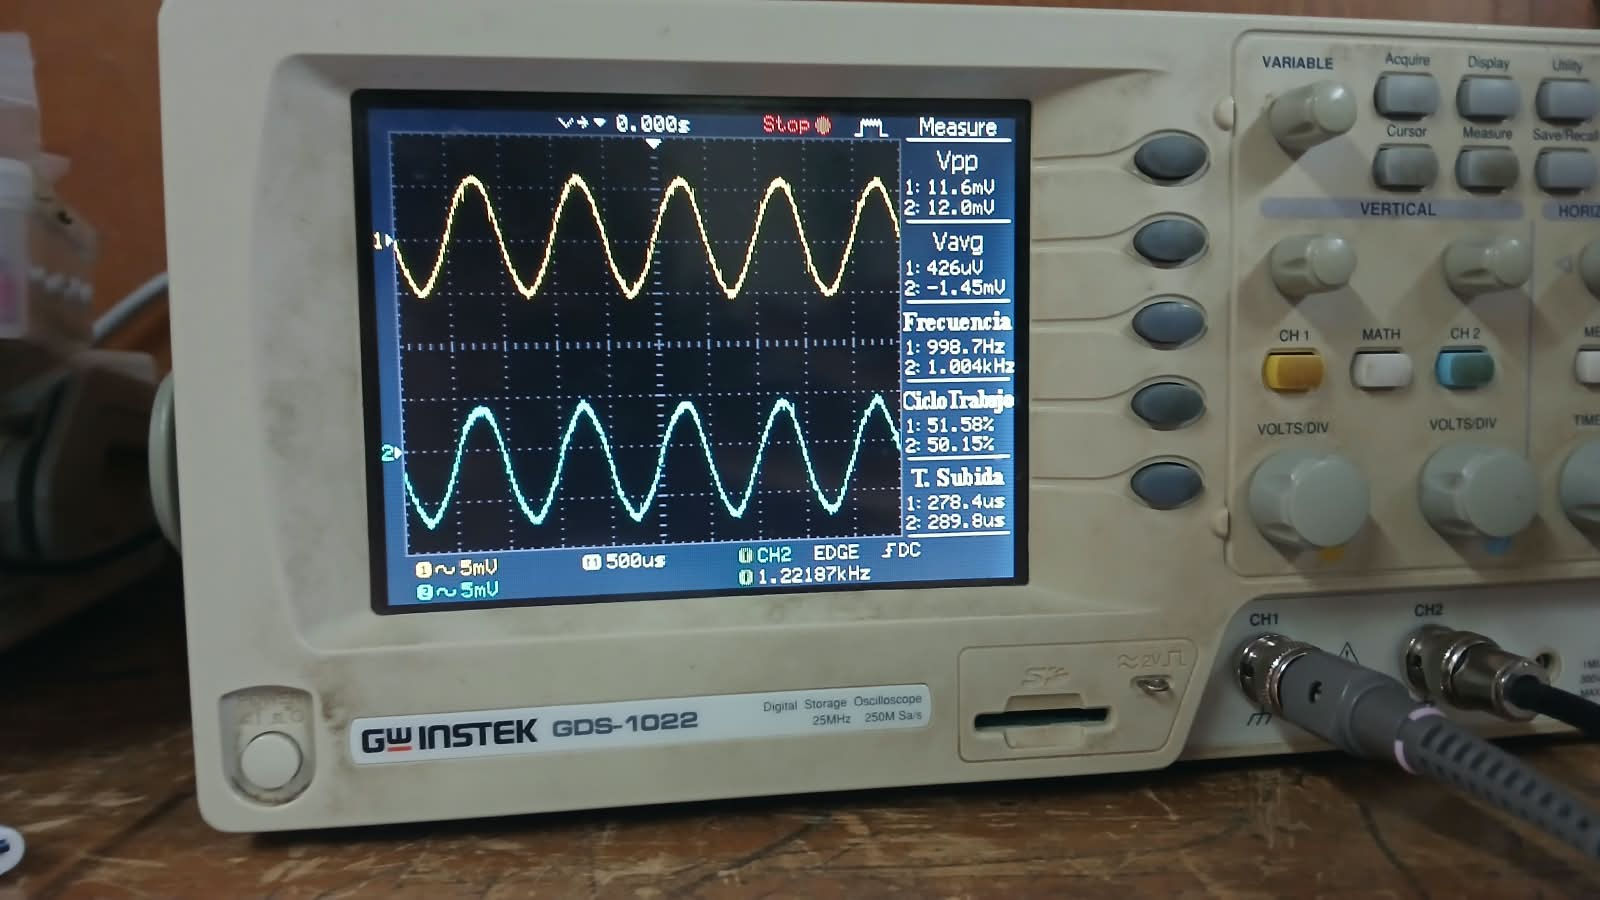
\includegraphics[width=0.8\textwidth]{FotosMed/Barrido de frecuencia/E1/1kzoom.jpeg}
    \caption{Pantalla del Osciloscopio}
    \label{fig:osciloscopioBArFrec}
\end{figure}

Se puede ver en \ref{fig:osciloscopioBArFrec}, la tension de entrada esta en el canal 2 del osciloscopio mientras que la salida se observa en el canal 1. El comportamiento es el esperado.

\subsubsection{Barrido de Etapa 1 y 2}
Al igual que con la medicion anterior y en la proxima, se uso la punta compensada conectada al osciloscopio para obtener las mediciones de tension

\begin{figure}[H]
    \centering
    % Primera minipage (ocupa el 45% del ancho de la página)
    \begin{minipage}{0.45\textwidth}
        \centering
        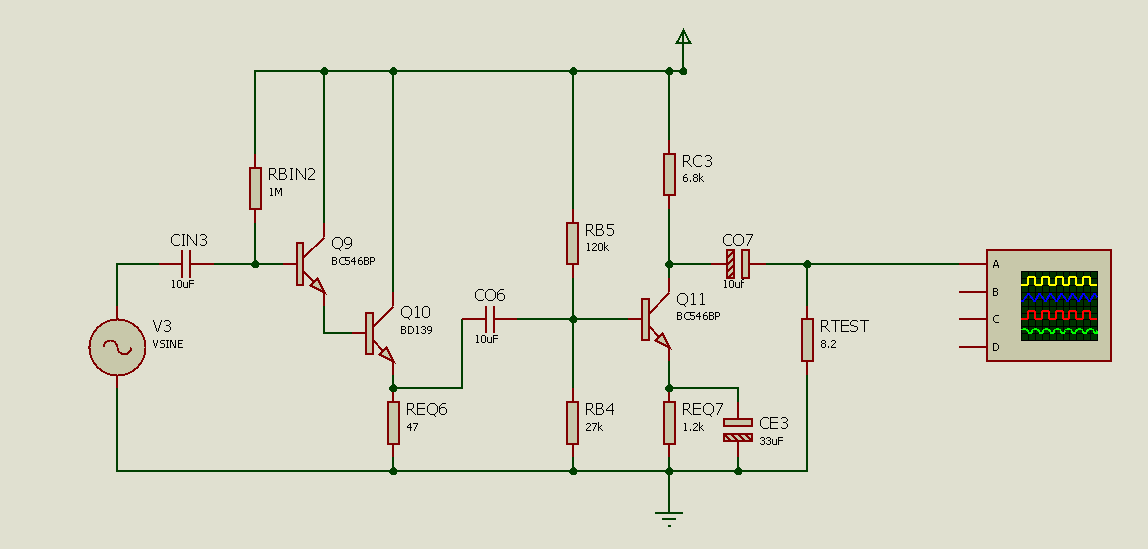
\includegraphics[width=\textwidth]{SetupMediciones/ZOUT/Zout12Cargada.png} % Ajusta el ancho al de la minipage
        \caption{Representacion esquematica.}
        \label{fig:esquematicofrec12}
    \end{minipage}
    \hfill % Relleno elástico para separar las imágenes
    % Segunda minipage (ocupa el 45% del ancho de la página)
    \begin{minipage}{0.45\textwidth}
        \centering
        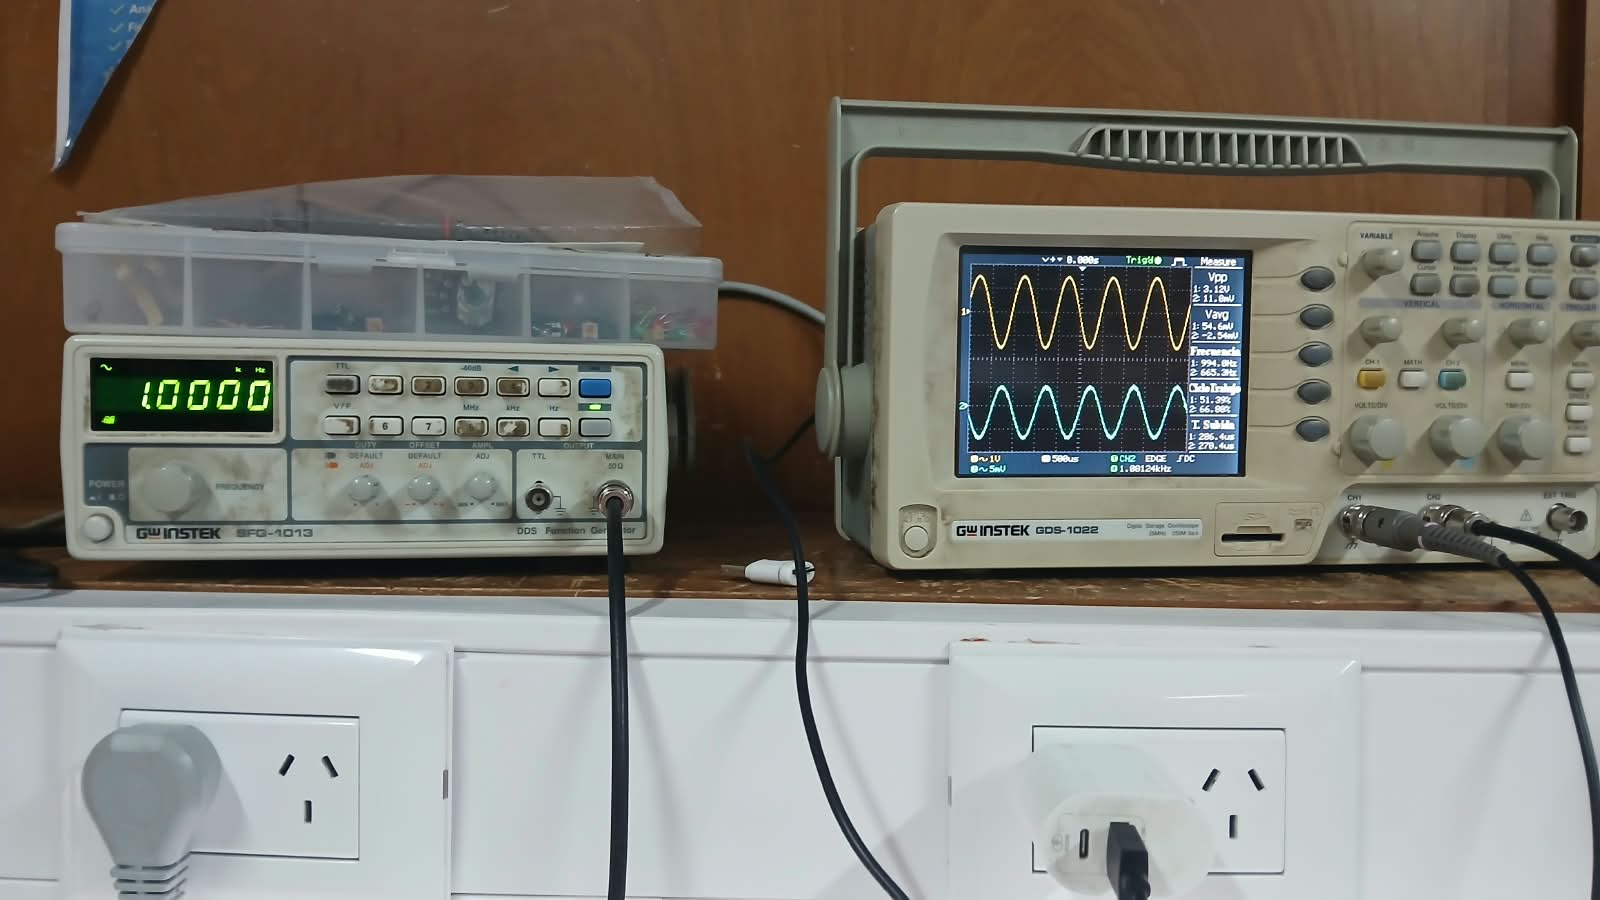
\includegraphics[width=\textwidth]{FotosMed/Barrido de frecuencia/E12/1k.jpeg}
        \caption{Imagen de la Medicion.}
        \label{fig:medicionfrec12}
    \end{minipage}
\end{figure}

\begin{figure}[H]
    \centering
    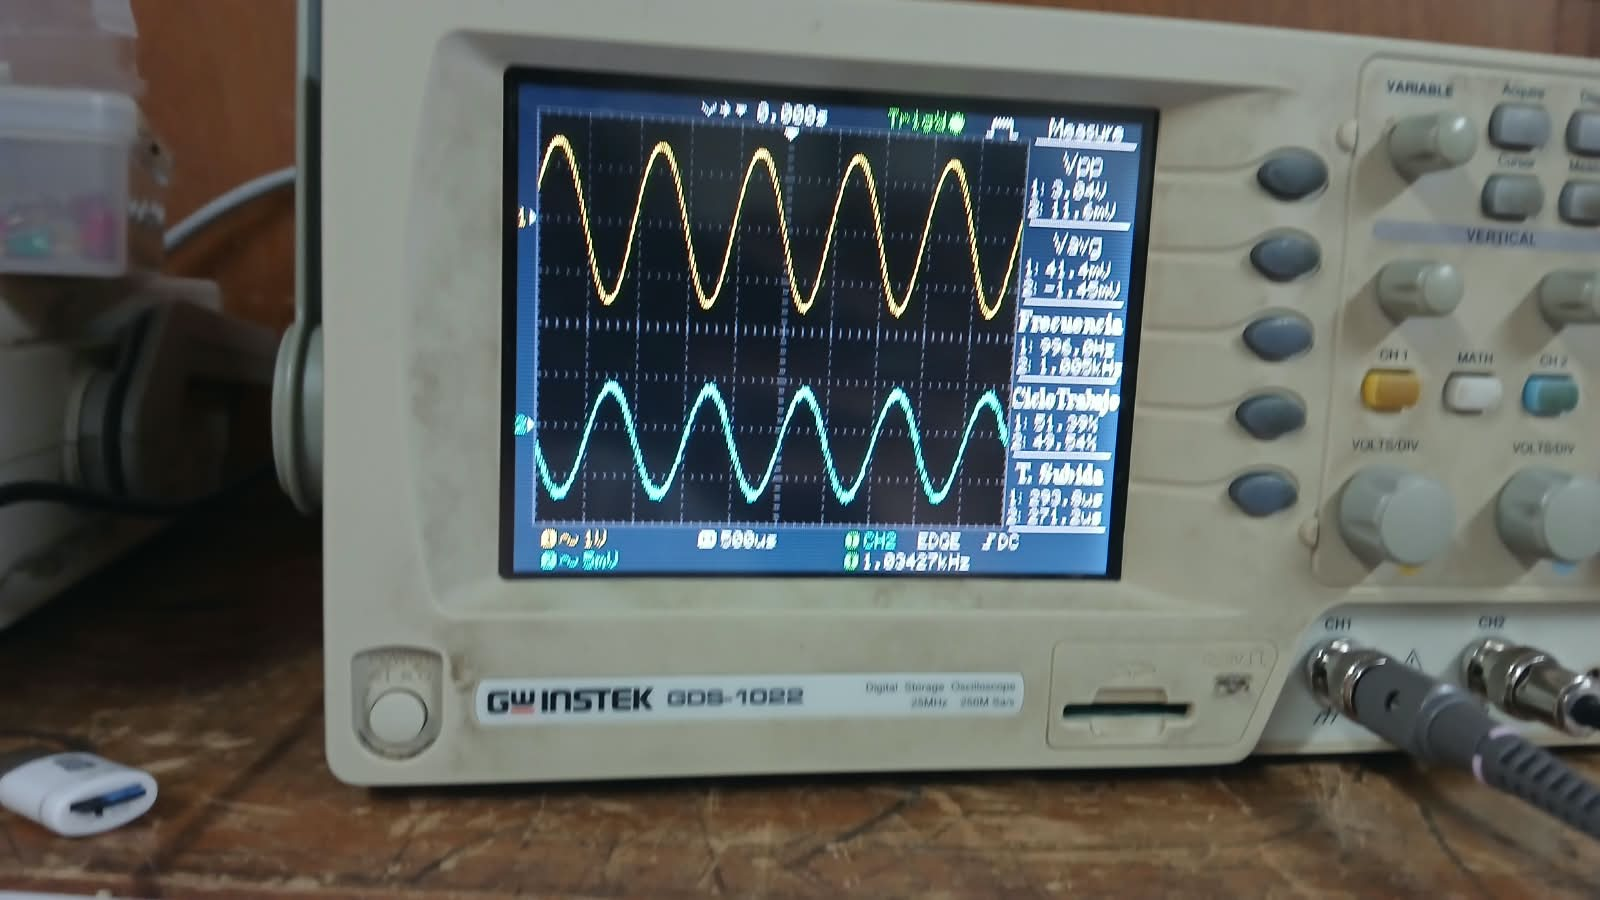
\includegraphics[width=0.8\textwidth]{FotosMed/Barrido de frecuencia/E12/1kzoom.jpeg}
    \caption{Pantalla del Osciloscopio}
    \label{fig:osciloscopiofrec12}
\end{figure}

Se puede ver en \ref{fig:osciloscopiofrec12} que la entrada esta conectada al canal 2 mientras que la salida al Canal 1, en estas etapas ya se evidencia la contundente ganancia.

\subsubsection{Barrido en circuito completo}
Sin casi variaciones, la medicion es reaizada observando la salida del circuito completo.

\begin{figure}[H]
    \centering
    % Primera minipage (ocupa el 45% del ancho de la página)
    \begin{minipage}{0.45\textwidth}
        \centering
        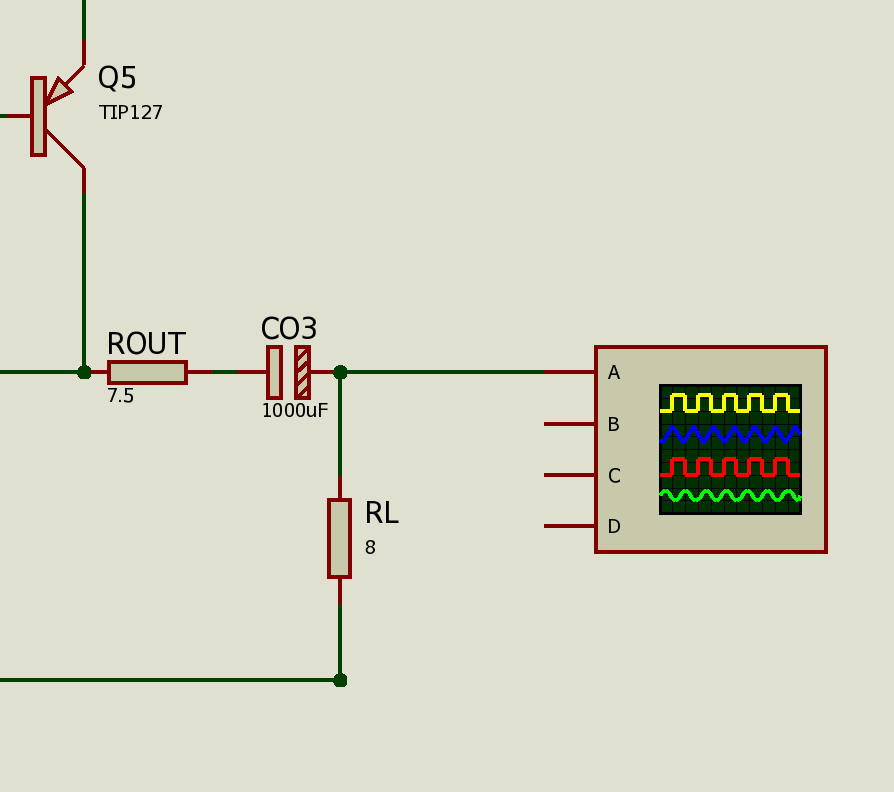
\includegraphics[width=\textwidth]{SetupMediciones/ZOUT/ZoutCarga.png} % Ajusta el ancho al de la minipage
        \caption{Representacion esquematica.}
        \label{fig:esquematicofrectotal}
    \end{minipage}
    \hfill % Relleno elástico para separar las imágenes
    % Segunda minipage (ocupa el 45% del ancho de la página)
    \begin{minipage}{0.45\textwidth}
        \centering
        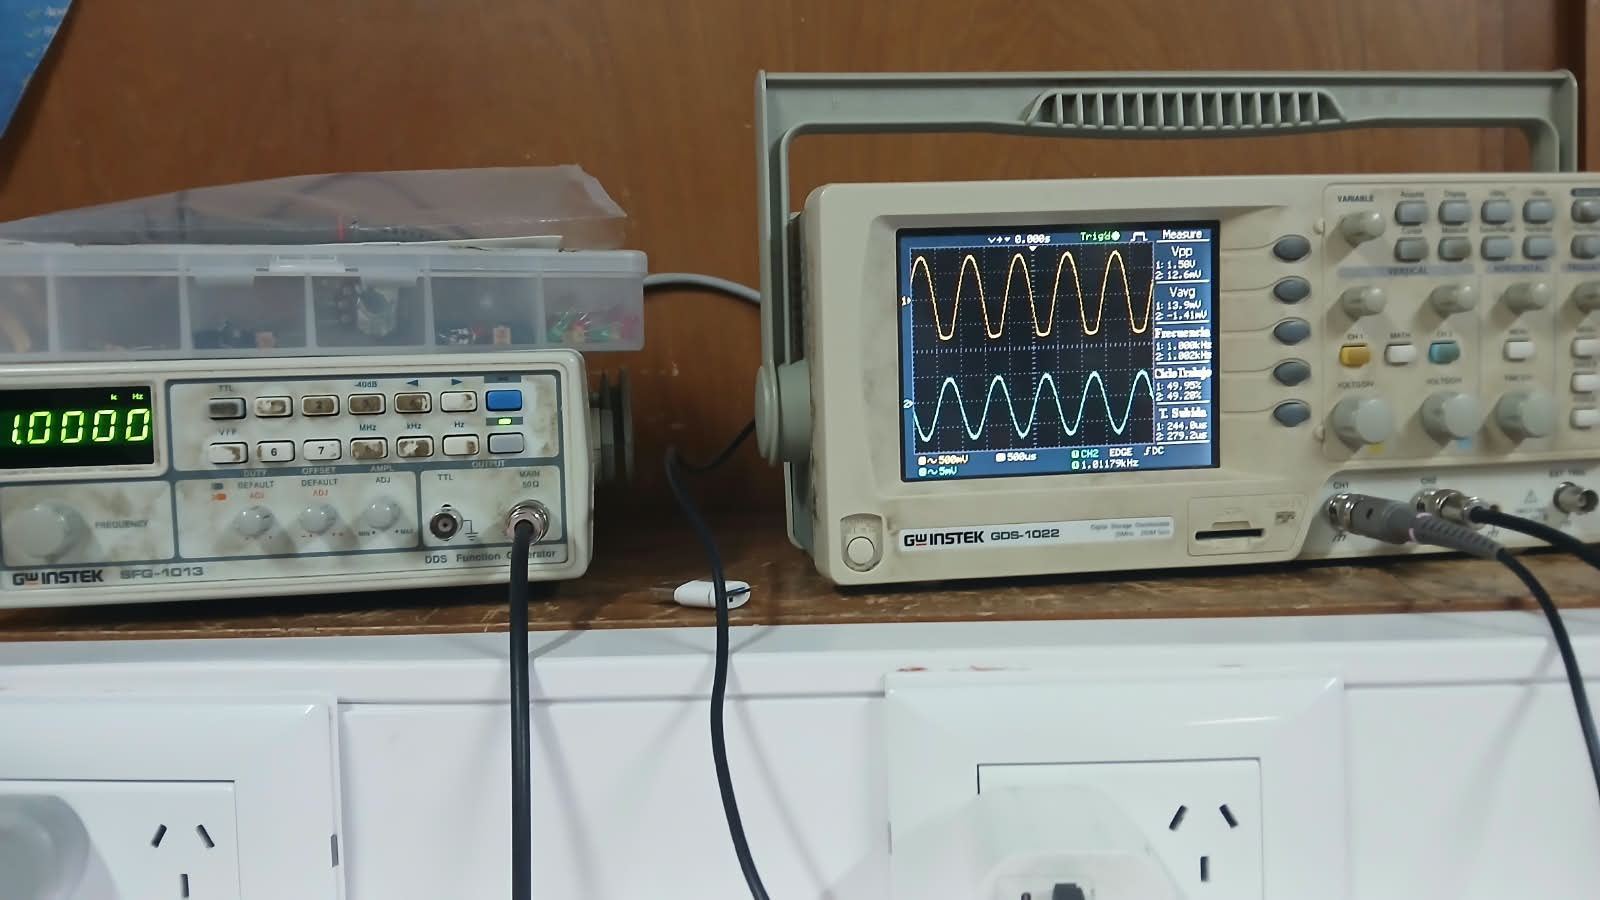
\includegraphics[width=\textwidth]{FotosMed/Barrido de frecuencia/Completo/1khz.jpeg}
        \caption{Imagen de la Medicion.}
        \label{fig:medicionfrectotal}
    \end{minipage}
\end{figure}

\begin{figure}[H]
    \centering
    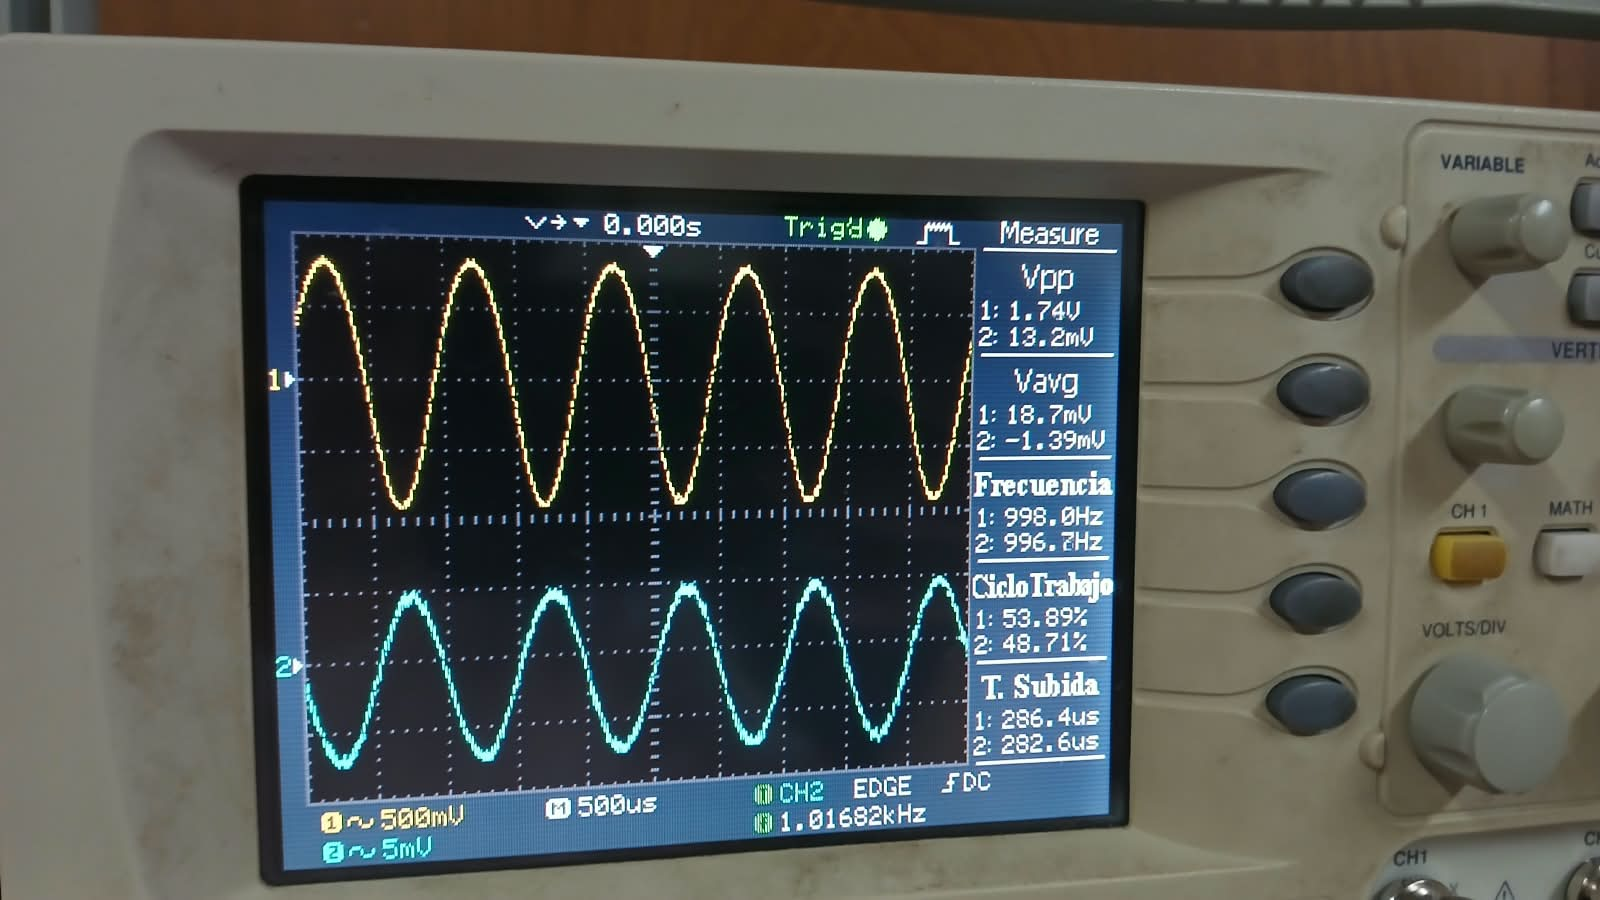
\includegraphics[width=0.8\textwidth]{FotosMed/Barrido de frecuencia/Completo/1khzzoom.jpeg}
    \caption{Pantalla del Osciloscopio}
    \label{fig:osciloscopiofrectotal}
\end{figure}

Se puede ver en \ref{fig:osciloscopiofrectotal} que la entrada esta conectada al canal 2 mientras que la salida al Canal 1, la ganancia disminuyo a la mitad en comparacion a la medicion anterior.

\subsection{Total Harmonic Distorsion}
Con la misma distribucion dada en el barrido de frecuencia, en este caso se utilizó la funcion de obtener la Transformada Rapida de Fourier (FFT) del osciloscopio para realizar los calculos de THD mediante:

\[
\mathrm{THD} = \frac{\sqrt{V_2^2 + V_3^2 + V_4^2 + \cdots + V_n^2}}{V_1}
\]

Como se dijo anteriormente, se midio en
- Etapa 1(Darlington)
- Etapa 1 y 2
- Circuito Completo

\subsubsection{FFT de Etapa 1}
Utilizando la punta compensada conectada al osciloscopio se obtuvo la salida de la etapa 1 y se aplico la FFT, una vez impresa en la pantalla se realizaron los calculos pertientes para determinar la THD.

\begin{figure}[H]
    \centering
    % Primera minipage (ocupa el 45% del ancho de la página)
    \begin{minipage}{0.45\textwidth}
        \centering
        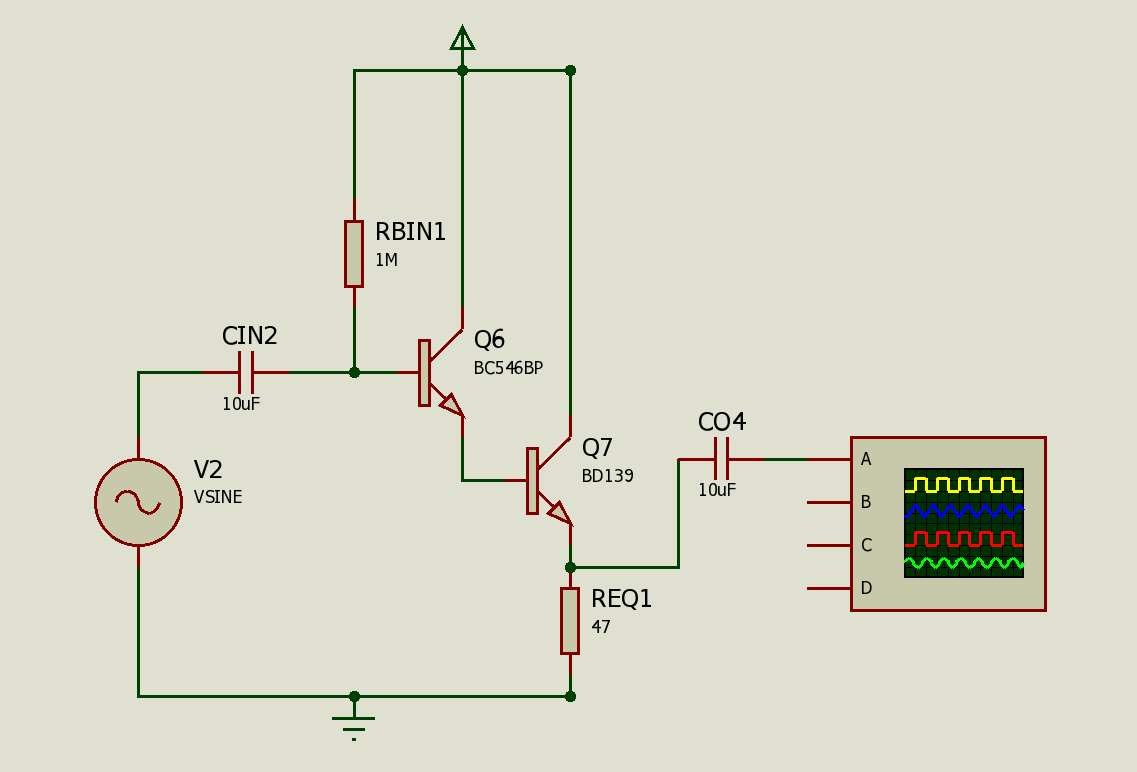
\includegraphics[width=\textwidth]{SetupMediciones/ZOUT/ZoutDARSinCarga.png} % Ajusta el ancho al de la minipage
        \caption{Representacion esquematica.}
        \label{fig:esquematicoFFT1}
    \end{minipage}
    \hfill % Relleno elástico para separar las imágenes
    % Segunda minipage (ocupa el 45% del ancho de la página)
    \begin{minipage}{0.45\textwidth}
        \centering
        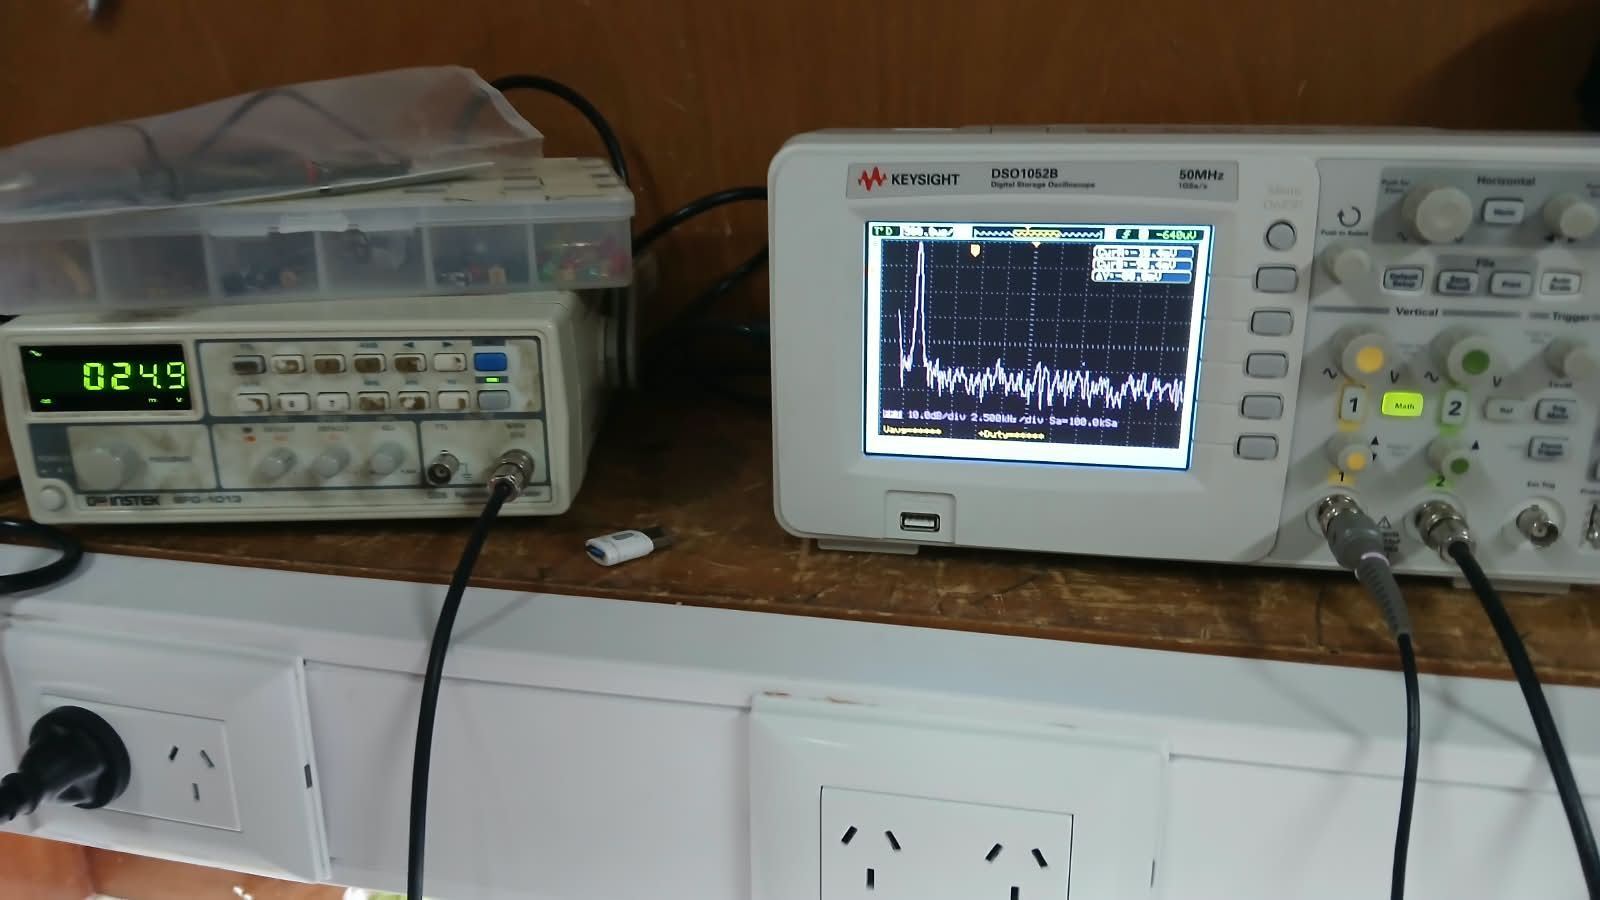
\includegraphics[width=\textwidth]{FotosMed/FFT/Dar/25dar.jpeg}
        \caption{Imagen de la Medicion.}
        \label{fig:medicionFFT1}
    \end{minipage}
\end{figure}

\begin{figure}[H]
    \centering
    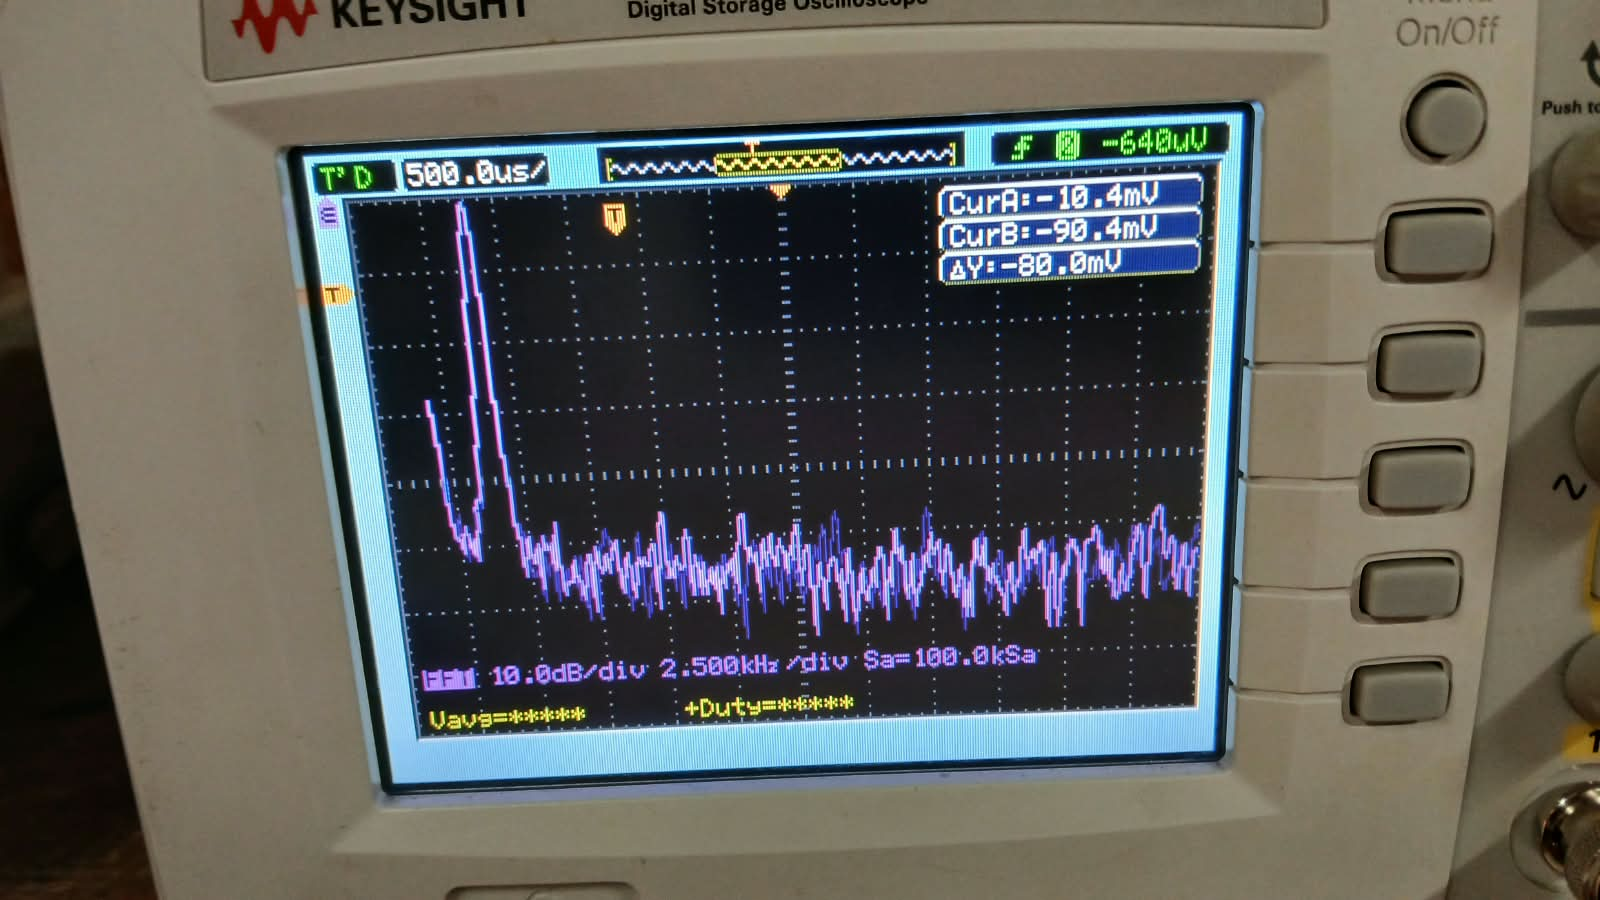
\includegraphics[width=0.8\textwidth]{FotosMed/FFT/Dar/25darzoom.jpeg}
    \caption{Pantalla del Osciloscopio}
    \label{fig:osciloscopioFFT1}
\end{figure}

Se puede ver en la Figura \ref{fig:osciloscopioFFT1}, la de entrada esta en el canal 2 del osciloscopio mientras que la salida se observa en el canal 1.No se observa casi distorsion en esta primer etapa.

\subsubsection{Barrido de Etapa 1 y 2}
Aqui se conectan los jumpers necesarios y se cambia la posicion de la punta a la salida de la etapa 2.

\begin{figure}[h]
    \centering
    % Primera minipage (ocupa el 45% del ancho de la página)
    \begin{minipage}{0.45\textwidth}
        \centering
        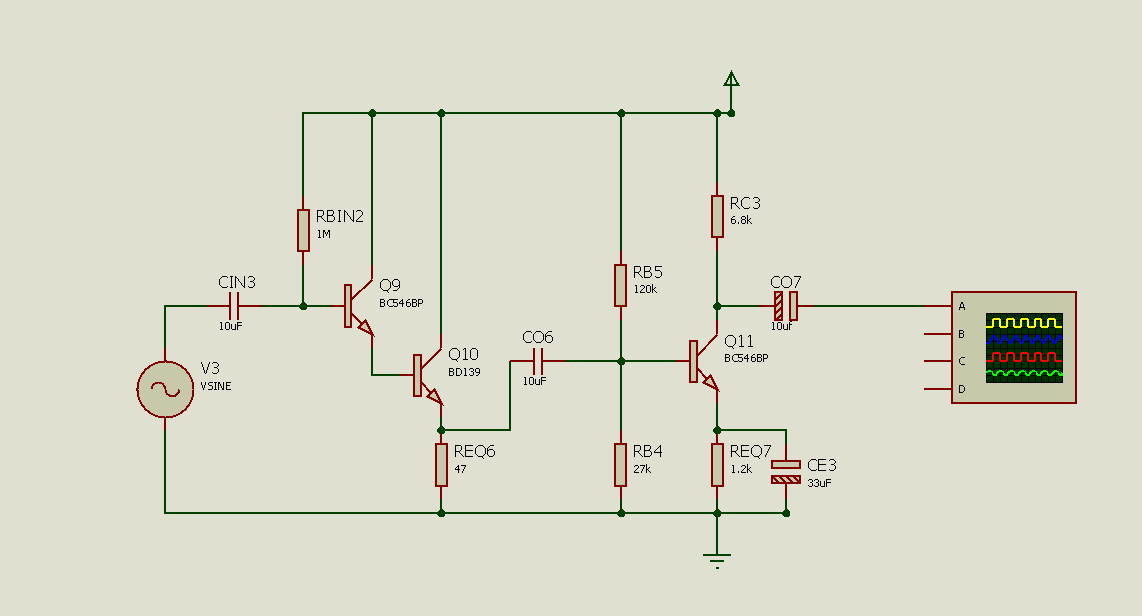
\includegraphics[width=\textwidth]{SetupMediciones/ZOUT/Zout12VACIO.png} % Ajusta el ancho al de la minipage
        \caption{Representacion esquematica.}
        \label{fig:esquematicpFFT12}
    \end{minipage}
    \hfill % Relleno elástico para separar las imágenes
    % Segunda minipage (ocupa el 45% del ancho de la página)
    \begin{minipage}{0.45\textwidth}
        \centering
        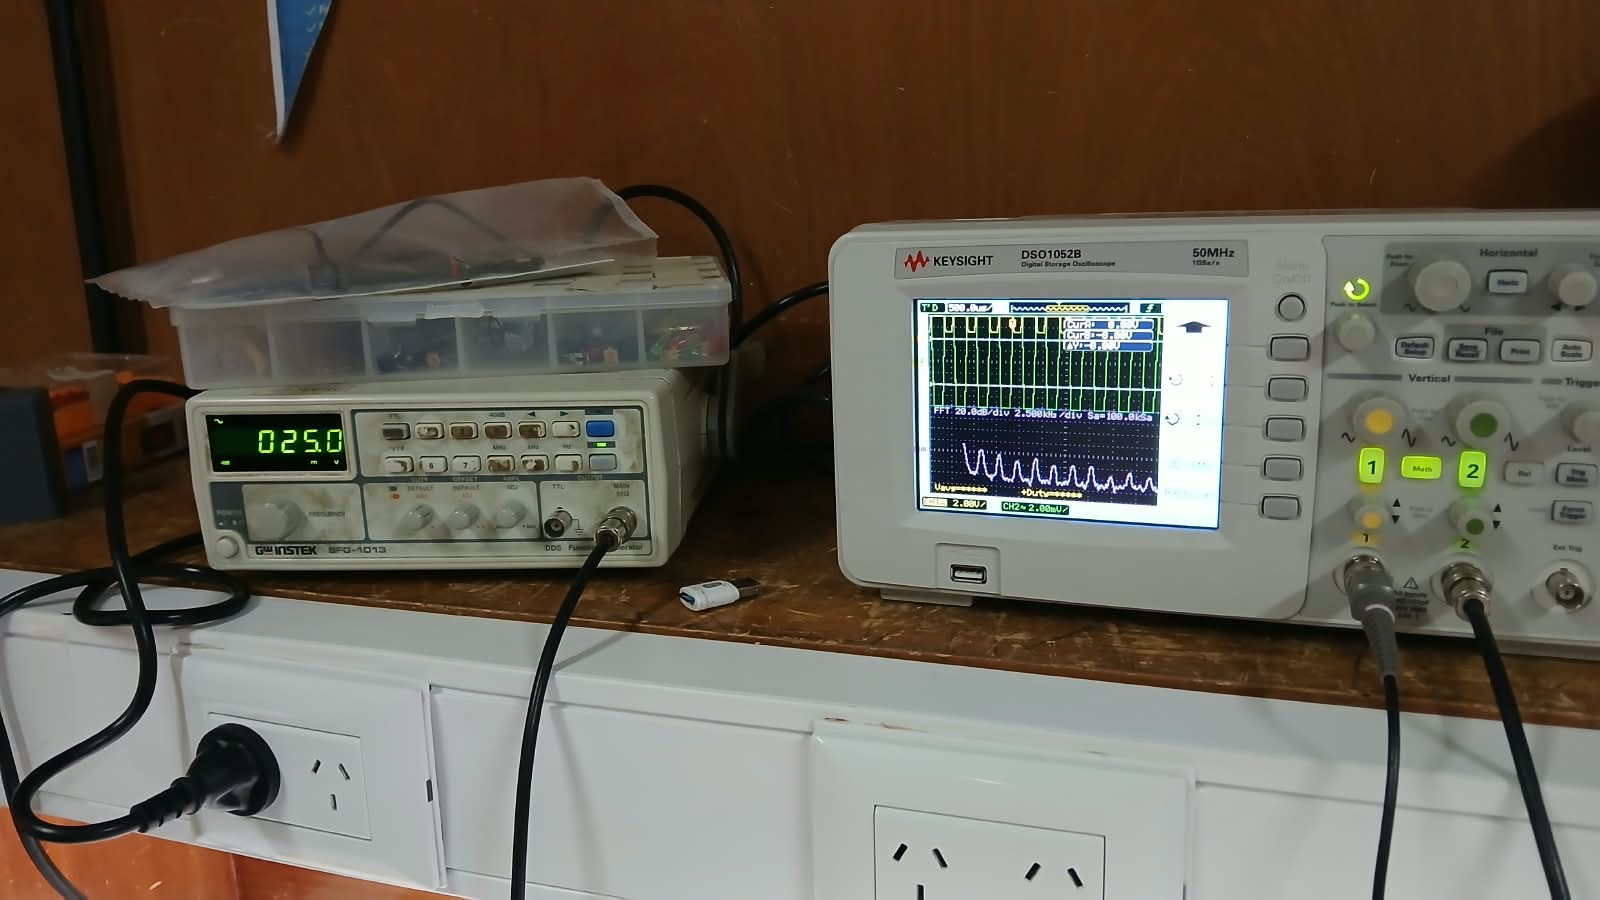
\includegraphics[width=\textwidth]{FotosMed/FFT/E12/25e12.jpeg}
        \caption{Imagen de la Medicion.}
        \label{fig:medicionFFT12}
    \end{minipage}
\end{figure}

\begin{figure}[H]
    \centering
    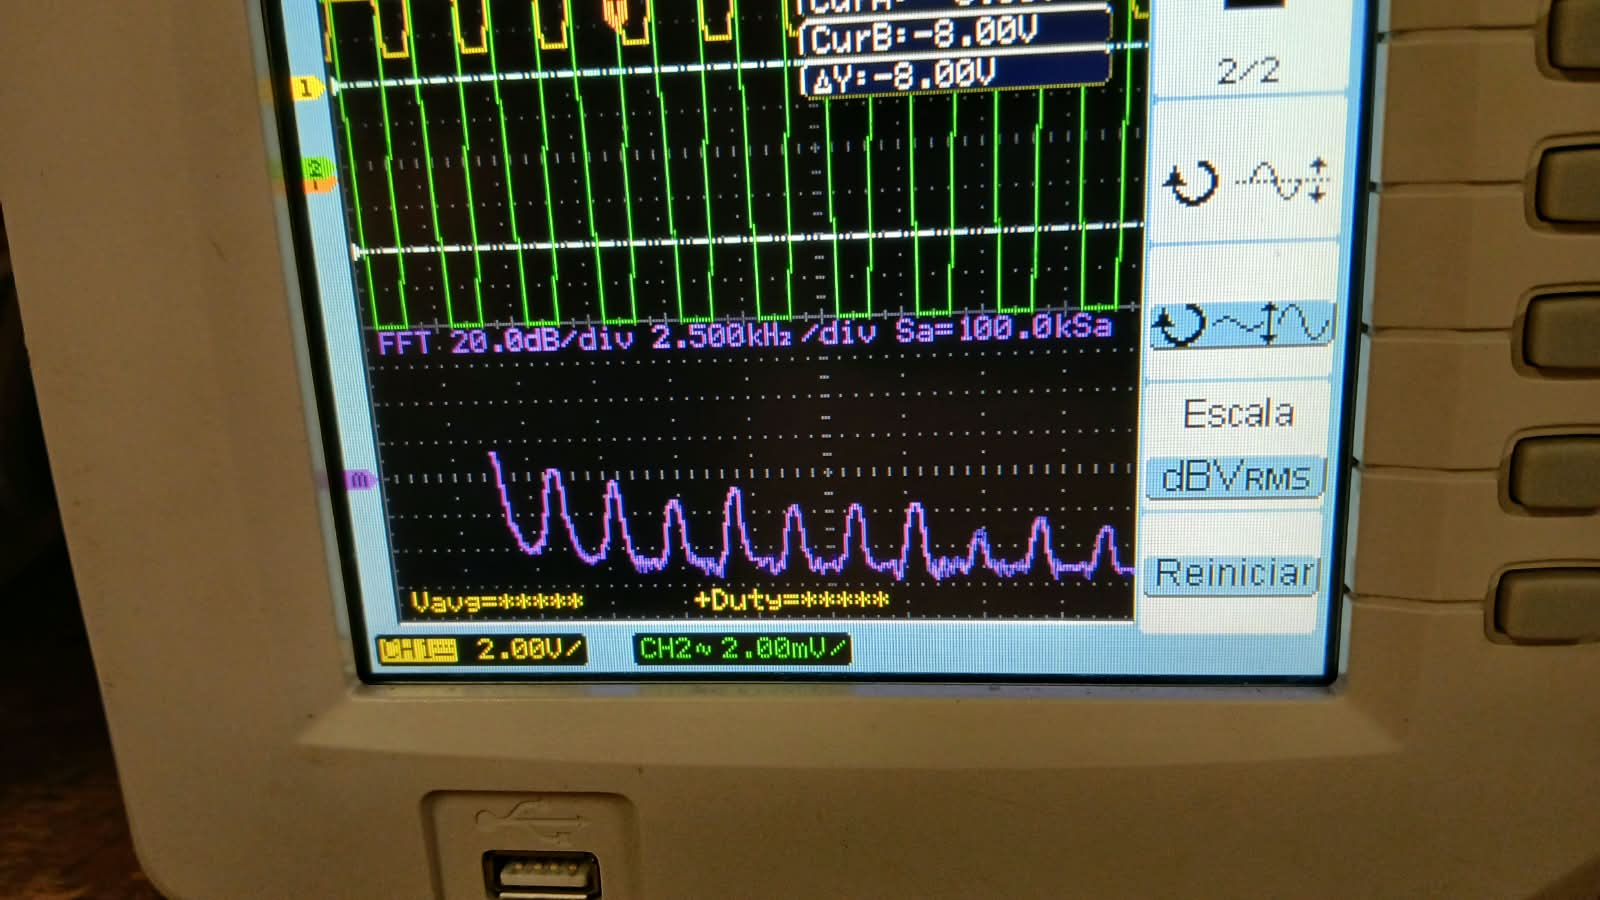
\includegraphics[width=0.8\textwidth]{FotosMed/FFT/E12/25e12zoom.jpeg}
    \caption{Pantalla del Osciloscopio}
    \label{fig:osciloscopioFFT12}
\end{figure}

Se puede ver en \ref{fig:osciloscopioFFT12} como la distorsión toma protagonismo evidenciandose en los picos de amplitud en frecuencias multiplos de 2Khz.

\subsubsection{FFT de circuito completo}
Con todos los jumpers conectados, se evalua la FFT del circuito final en la pantalla del osciloscopio 

\begin{figure}[H]
    \centering
    % Primera minipage (ocupa el 45% del ancho de la página)
    \begin{minipage}{0.45\textwidth}
        \centering
        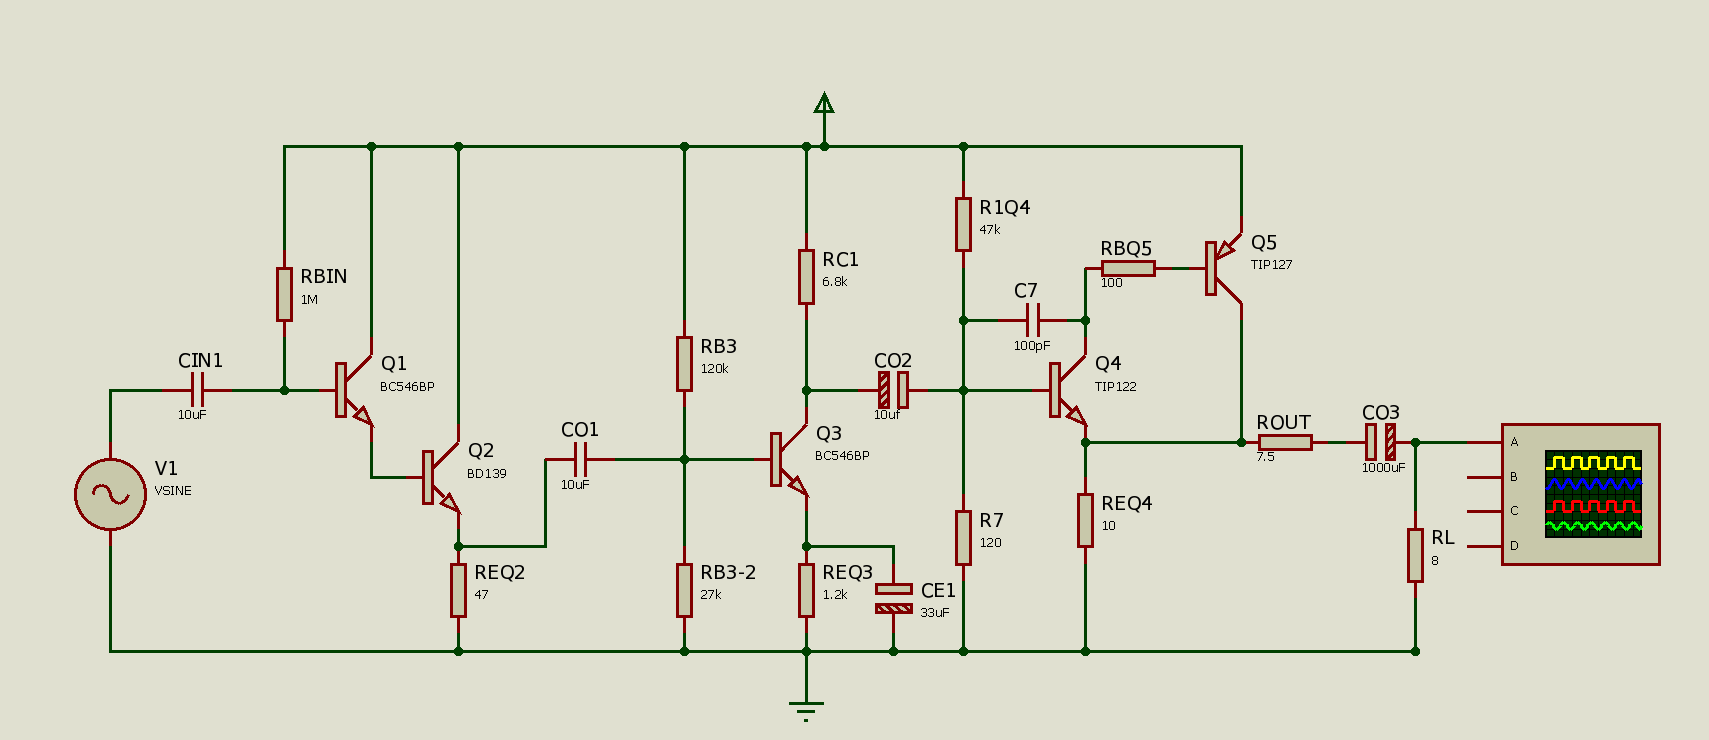
\includegraphics[width=\textwidth]{SetupMediciones/TensionesCorrientes/BarridoDeFrecuencia.png} % Ajusta el ancho al de la minipage
        \caption{Representacion esquematica.}
        \label{fig:esquematicoFFTCompleto}
    \end{minipage}
    \hfill % Relleno elástico para separar las imágenes
    % Segunda minipage (ocupa el 45% del ancho de la página)
    \begin{minipage}{0.45\textwidth}
        \centering
        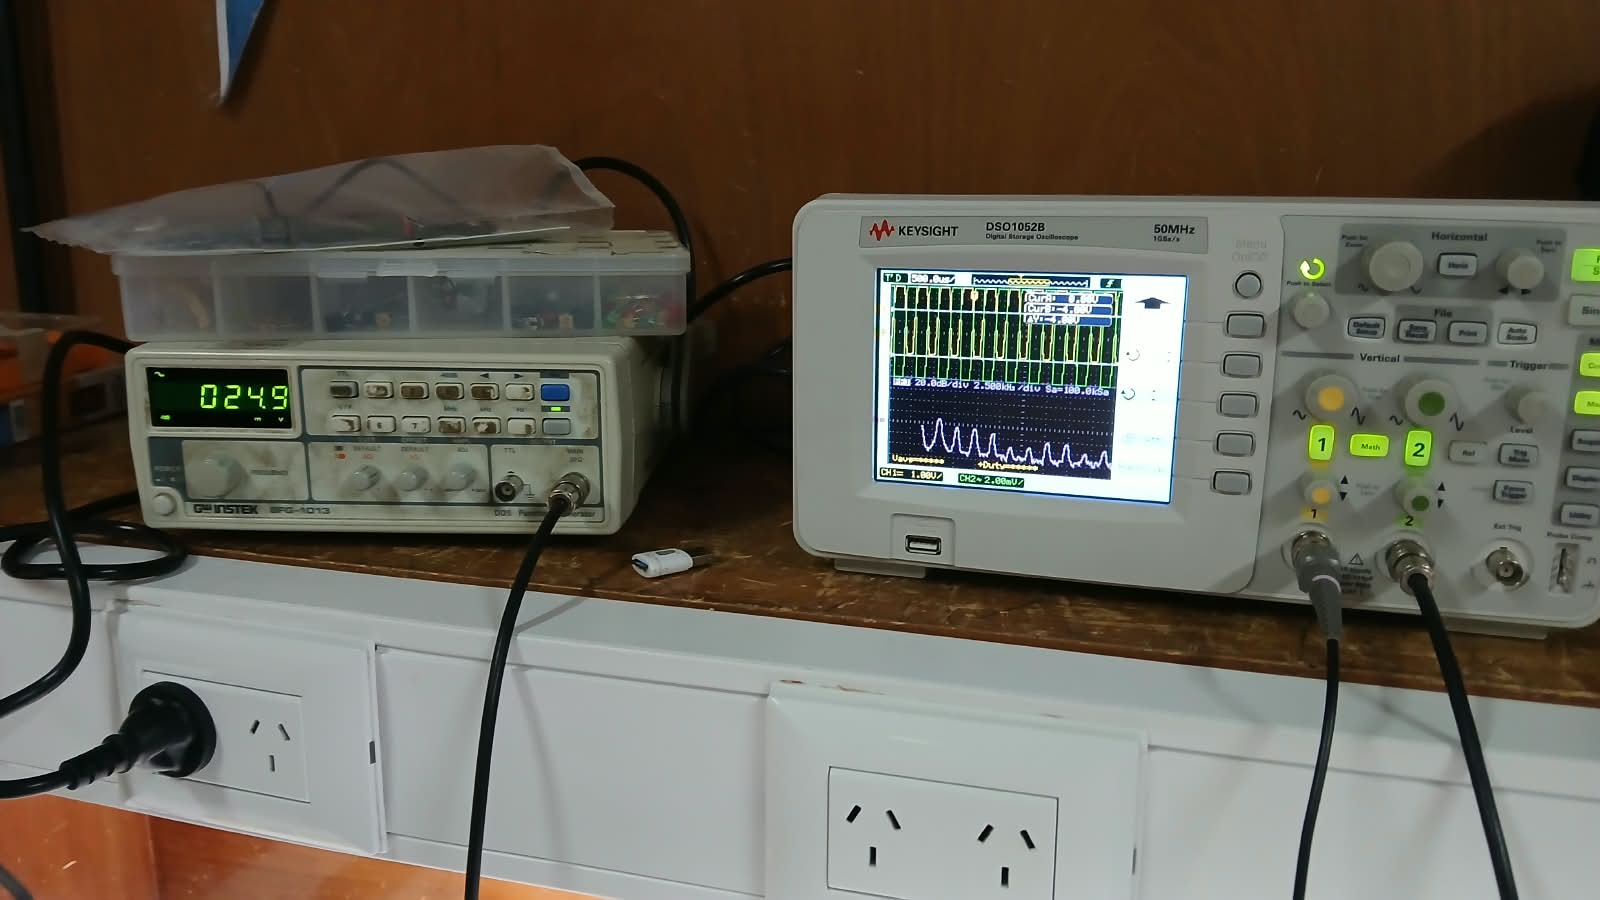
\includegraphics[width=\textwidth]{FotosMed/FFT/Completo/25com.jpeg}
        \caption{Imagen de la Medicion.}
        \label{fig:medicionFFTCompleto}
    \end{minipage}
\end{figure}

\begin{figure}[H]
    \centering
    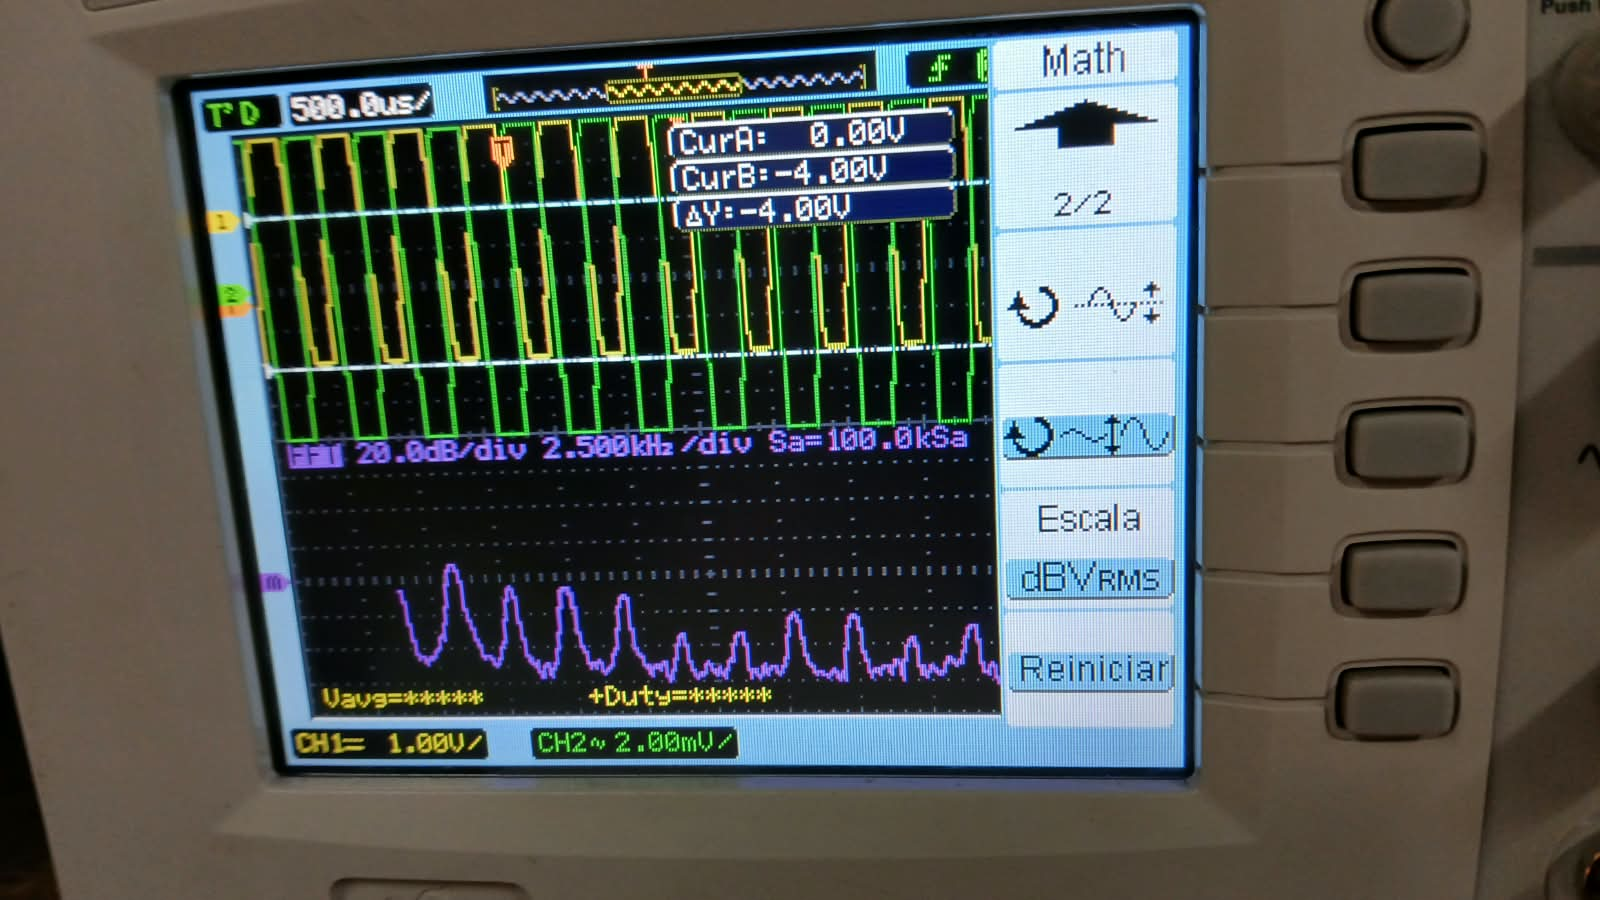
\includegraphics[width=0.8\textwidth]{FotosMed/FFT/Completo/25comzoom.jpeg}
    \caption{Pantalla del Osciloscopio}
    \label{fig:osciloscopioFFTCompleto}
\end{figure}

Se puede ver en \ref{fig:osciloscopioFFTCompleto} una gran distorsion dado que el dispositivo empieza a recortar el semiciclo inferior de la onda.

\subsection{Impedancia De Salida y de entrada}
A continuacion se vera el método de medicion de las impedancias de salida y de entrada para las siguientes configuraciones

Se midio en:
- Etapa 1
- Etapa 1 y 2
- Circuito Completo

\subsubsection{Zout}
Para la medicion de impedancia de salida se trabajó en 2 partes para cada configuracion del equipo en pruebas, se midio la tensión a la salida en vacío y con carga conectada. Para todas las mediciones se utilizo una resistencia conocida de un orden de magnitud similar al esperado en la configuracion en medicion. Una vez obtenidas las mediciones se utilizó la siguiente ecuación:

\[
Z_{\mathrm{out}} = R_L \cdot \left( \frac{V_{\mathrm{vacio}} - V_{\mathrm{carga}}}{V_{\mathrm{carga}}} \right)
\]

Para representar las medicioens se usará como ejemplo la medición de impedancia de salida total.

\begin{figure}[H]
    \centering
    % Primera minipage (ocupa el 45% del ancho de la página)
    \begin{minipage}{0.45\textwidth}
        \centering
        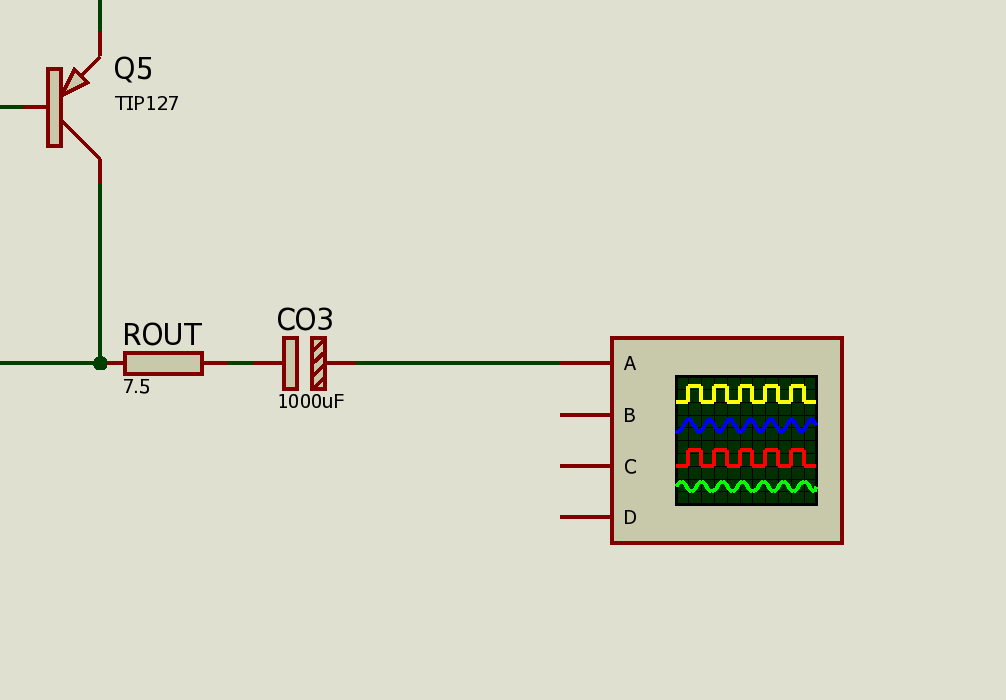
\includegraphics[width=\textwidth]{SetupMediciones/ZOUT/ZoutSinCarga.png} % Ajusta el ancho al de la minipage
        \caption{Representacion esquematica.}
        \label{fig:esquematicpZout}
    \end{minipage}
    \hfill % Relleno elástico para separar las imágenes
    % Segunda minipage (ocupa el 45% del ancho de la página)
    \begin{minipage}{0.45\textwidth}
        \centering
        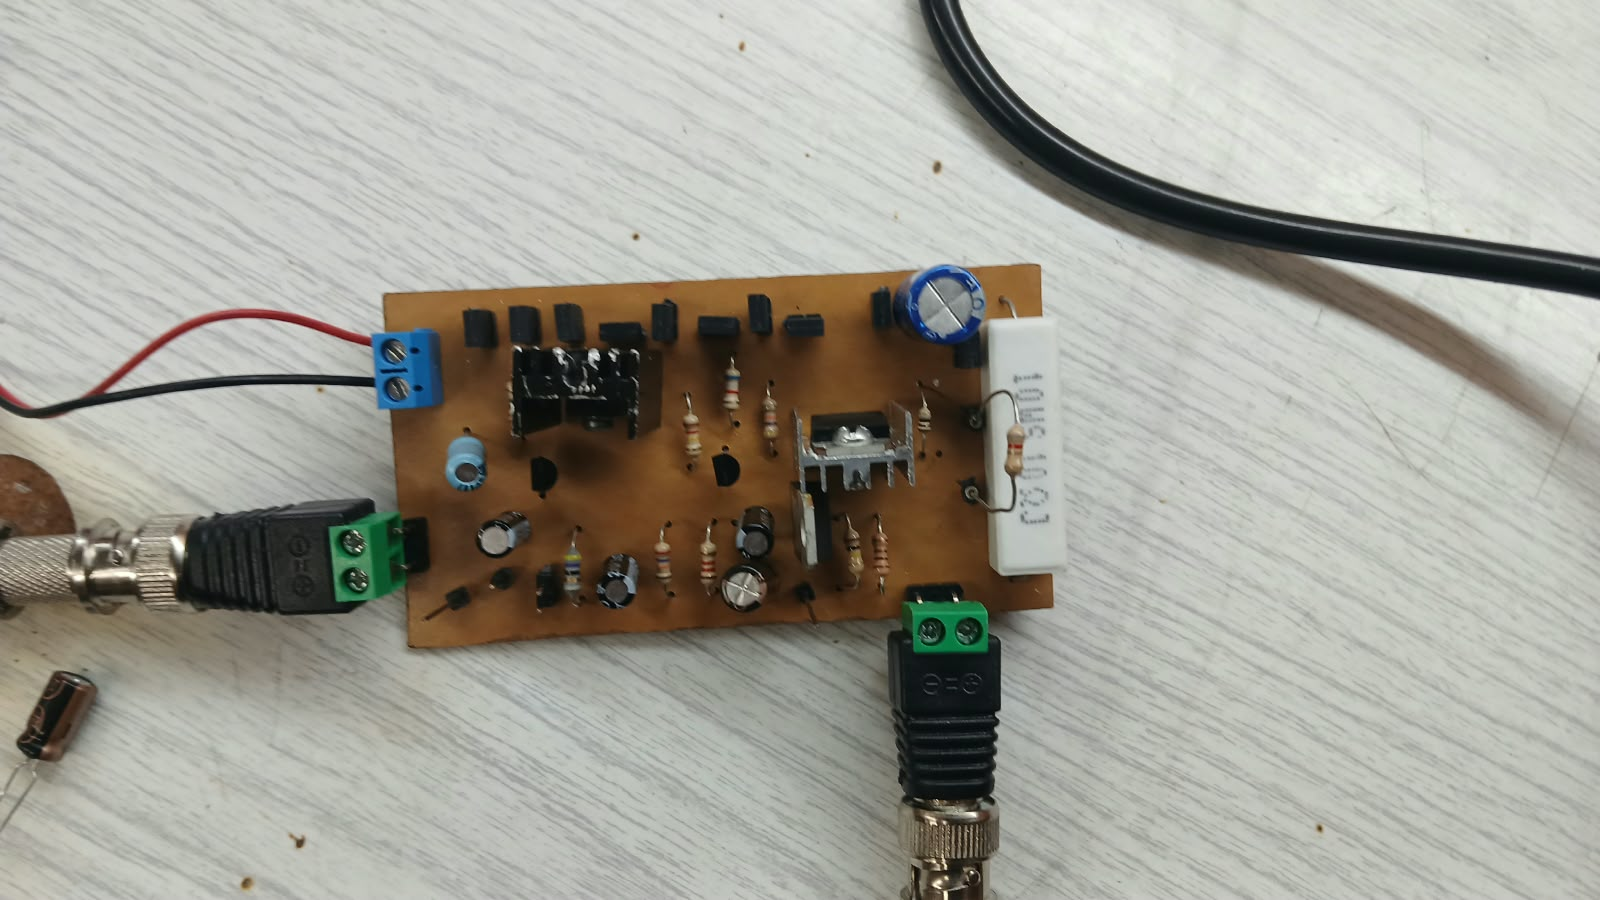
\includegraphics[width=\textwidth]{FotosMed/Impedancias/Zoutmed.jpeg}
        \caption{Setup de la Medicion.}
        \label{fig:medicionZout}
    \end{minipage}
\end{figure}

\begin{figure}[H]
    \centering
    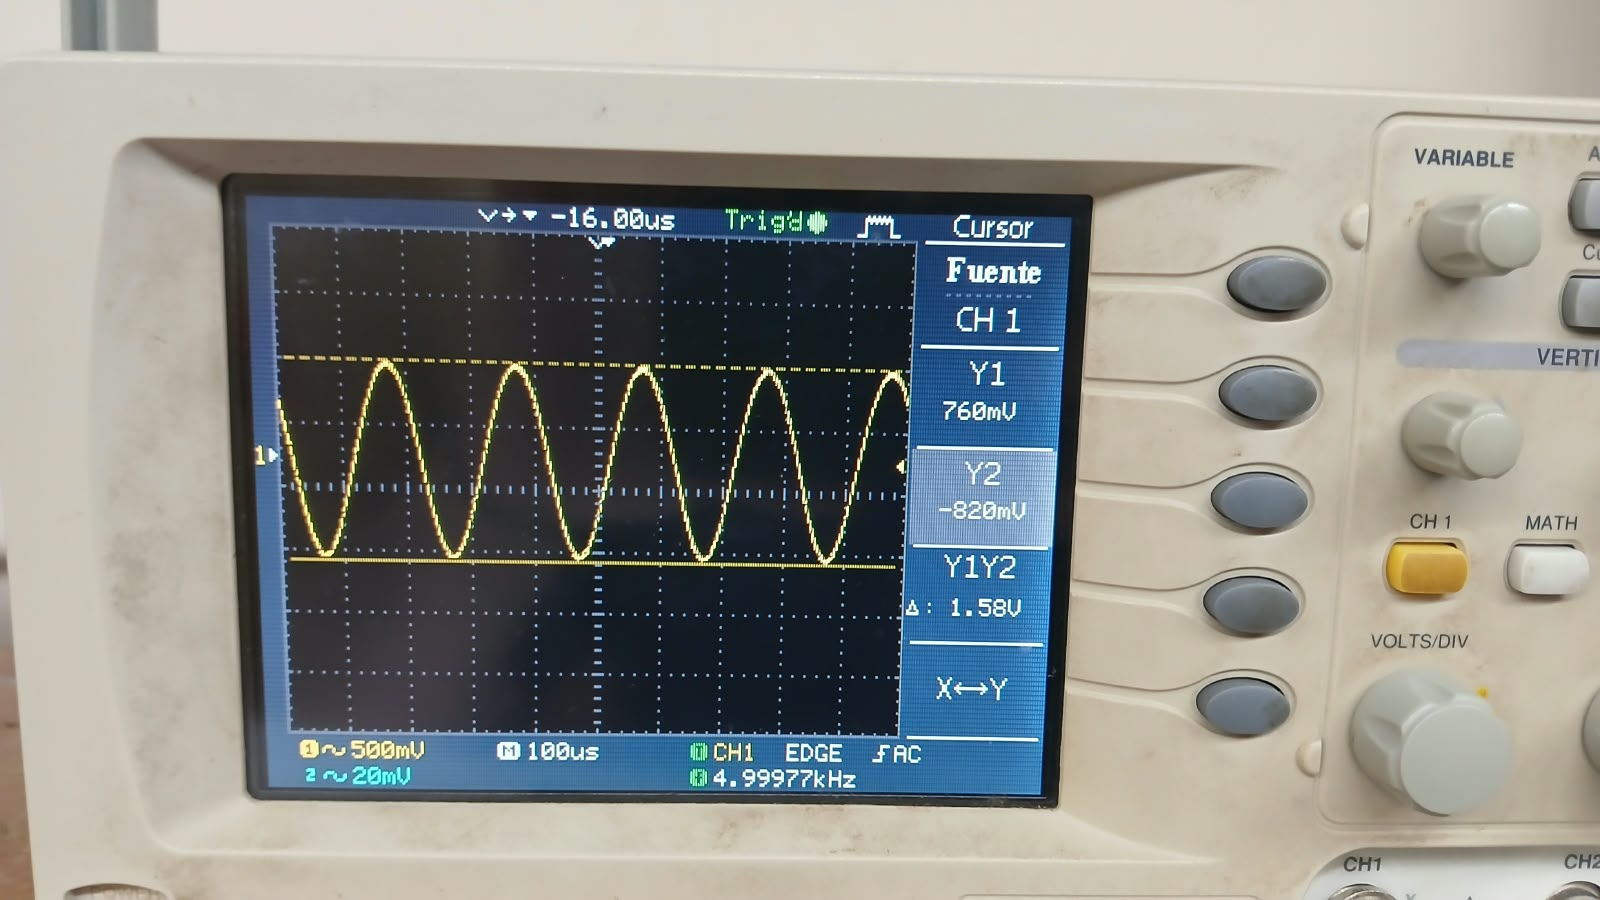
\includegraphics[width=0.8\textwidth]{FotosMed/Impedancias/Zout1.jpeg}
    \caption{Salida del Circuito en Vacio}
    \label{fig:osciloscopiozout}
\end{figure}

En \ref{fig:osciloscopiozout} se muestra el uso de cursores para la medición de tension de salida en vacio. Sigueinte a esta se realizo la medicion del circuito cargado con la Rl.

\begin{figure}[H]
    \centering
    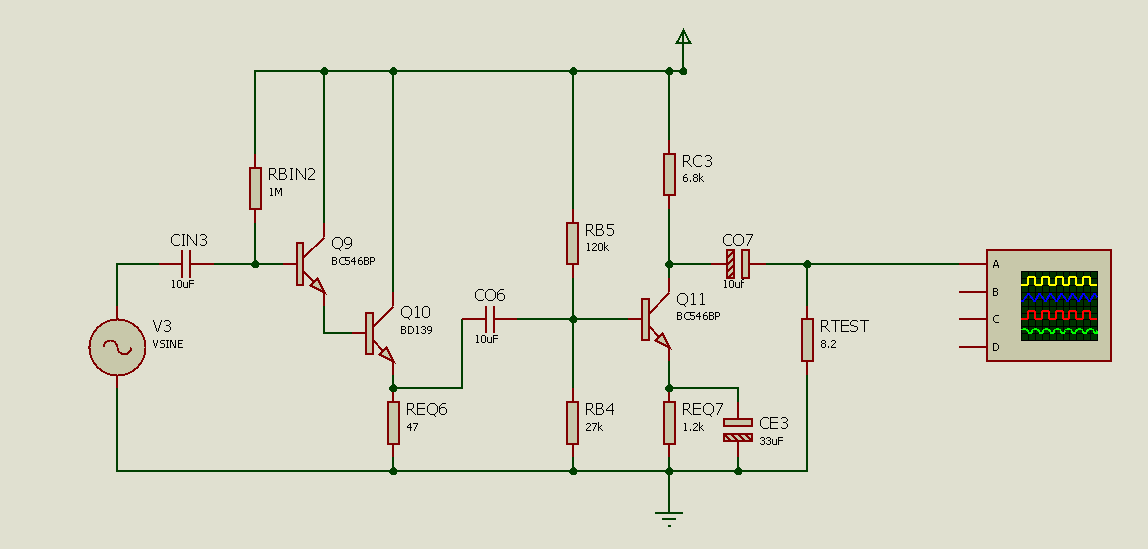
\includegraphics[width=0.8\textwidth]{SetupMediciones/ZOUT/Zout12Cargada.png}
    \caption{Esquema del Circuito Cargado}
    \label{fig:esquemaCargado}
\end{figure}


\begin{figure}[H]
    \centering
    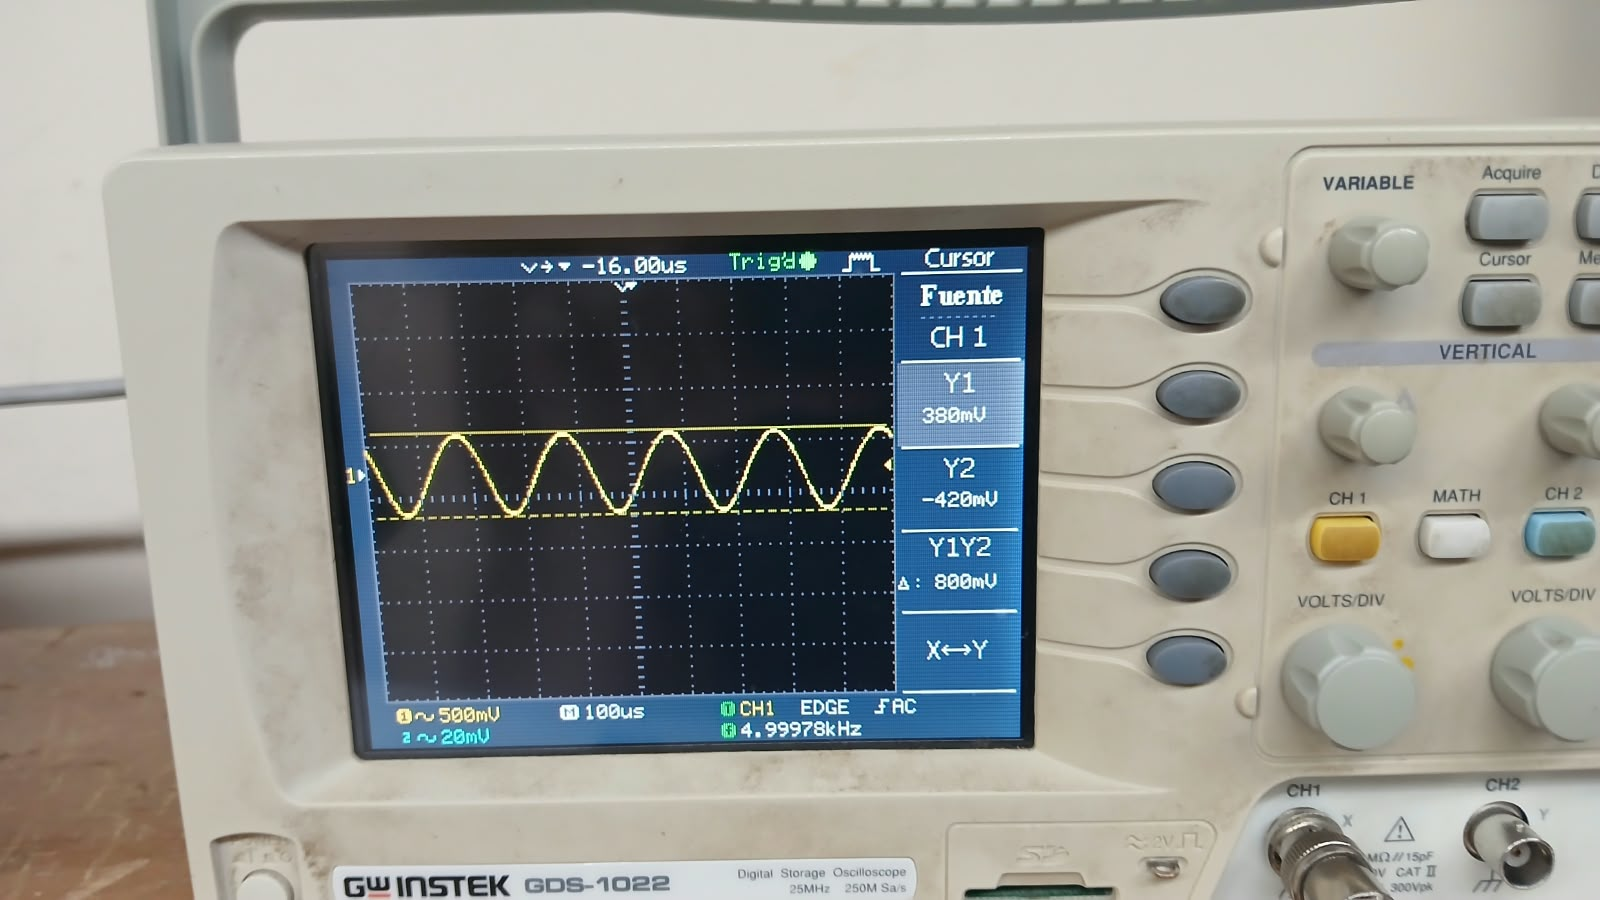
\includegraphics[width=0.8\textwidth]{FotosMed/Impedancias/Zout2.jpeg}
    \caption{Salida del Circuito Cargado}
    \label{fig:osciloscopio2}
\end{figure}

En \ref{fig:osciloscopio2} se muestra la salida del circuito cargado, evidenciandose una disminución de la amplitud de salida.

\subsection{Zin}
Para la medición de la impedancia de entrada el metodo fue diferente, se inyecto la señal atraves de una resistecnia en serie previa a la entrada de una magnitud similar a la impedancia esperada, dado que, si la tensión luego de la resistencia serie es la mitad que la proporcinaba por el generador, entonces la resistencia es exactamente igual a la Impedancia de entrada de la etapa bajo prueba.

Esto ocurre debido a el metodo de divisior de tension:
\[
V_{\mathrm{circuito}} = \frac{V_{\mathrm{gen}}}{2}
\]

Reemplazando esta igualdad en la ecuación original:

\[
\frac{V_{\mathrm{gen}}}{2} = V_{\mathrm{gen}} \cdot \left( \frac{Z_{\mathrm{in}}}{R_S + Z_{\mathrm{in}}} \right)
\]

Simplificando $V_{\mathrm{gen}}$ en ambos miembros dividiendo por $V_{\mathrm{gen}}$:

\[
\frac{1}{2} = \frac{Z_{\mathrm{in}}}{R_S + Z_{\mathrm{in}}}
\]

Se multiplica cruzado para despejar:

\[
R_S + Z_{\mathrm{in}} = 2 \cdot Z_{\mathrm{in}}
\]

Se resta $Z_{\mathrm{in}}$ en ambos lados:

\[
R_S = 2 \cdot Z_{\mathrm{in}} - Z_{\mathrm{in}}
\]

\[
R_S = Z_{\mathrm{in}}
\]

\[
V_{\mathrm{circuito}} = \frac{V_{\mathrm{gen}}}{2}
\]

Se utilizará de ejemplo la medicion de impedancia de entrada total.

\begin{figure}[H]
    \centering
    % Primera minipage (ocupa el 45% del ancho de la página)
    \begin{minipage}{0.45\textwidth}
        \centering
        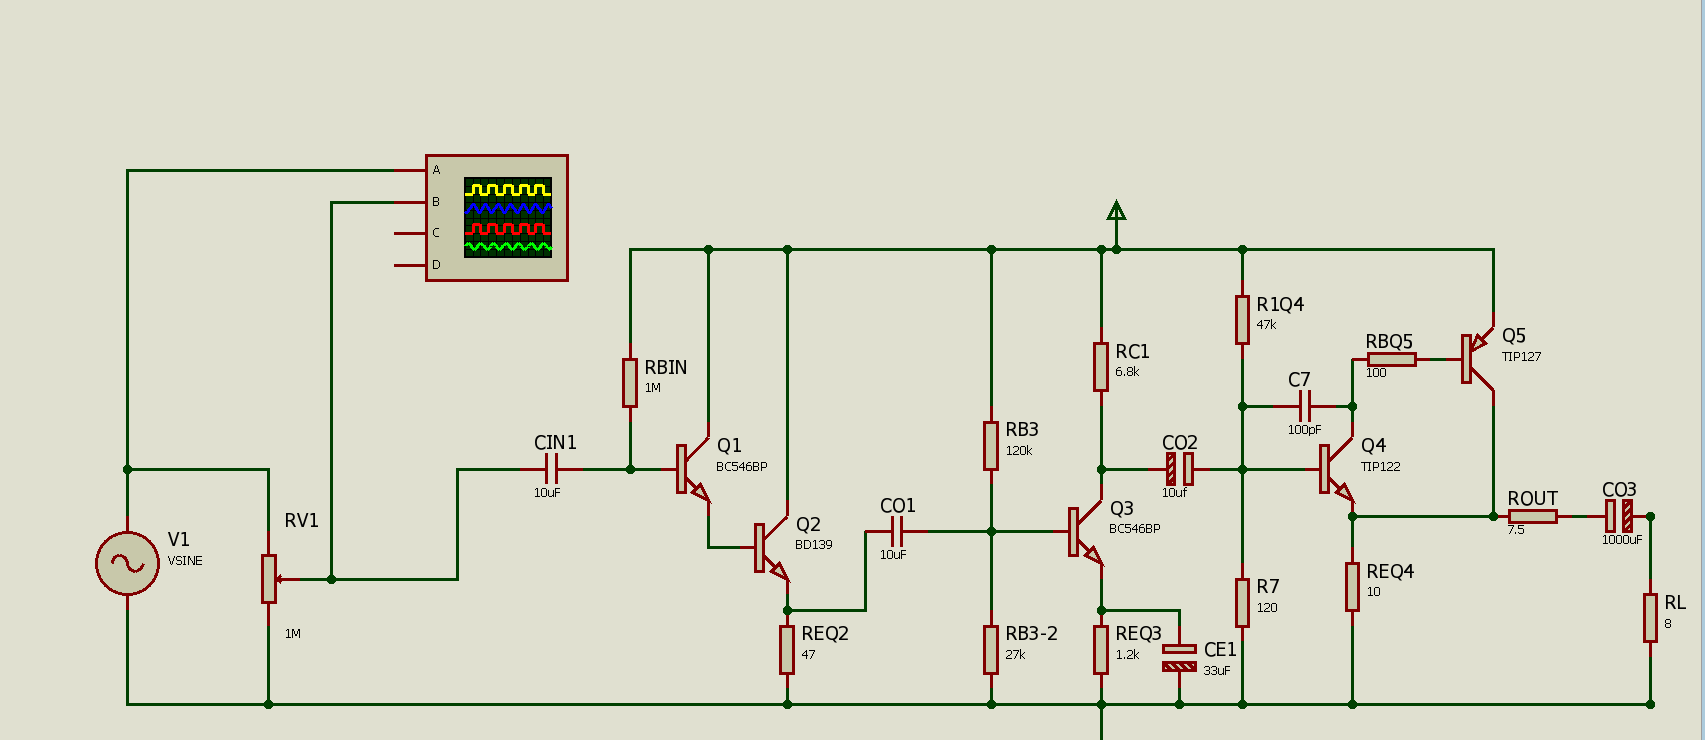
\includegraphics[width=\textwidth]{SetupMediciones/ZIN/ZinTotal.png} % Ajusta el ancho al de la minipage
        \caption{Representación esquemática.}
        \label{fig:esquematicpZin}
    \end{minipage}
    \hfill % Relleno elástico para separar las imágenes
    % Segunda minipage (ocupa el 45% del ancho de la página)
    \begin{minipage}{0.45\textwidth}
        \centering
        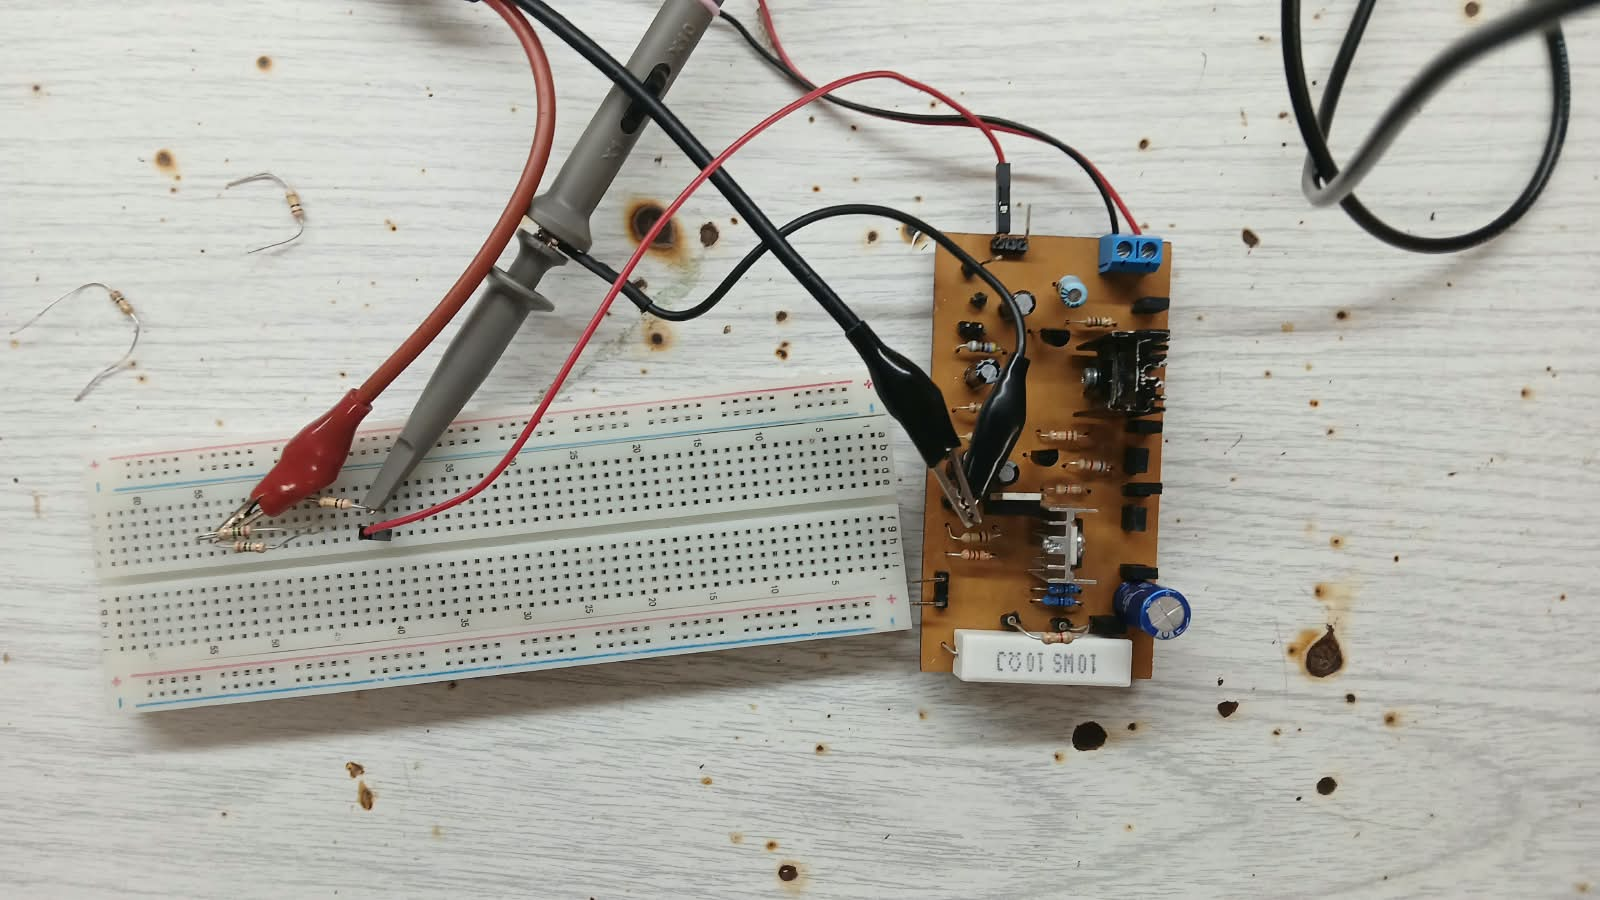
\includegraphics[width=\textwidth]{FotosMed/Impedancias/zinMed.jpeg}
        \caption{Imagen de la Medición.}
        \label{fig:medicionZin}
    \end{minipage}
\end{figure}

Se puede ver en \ref{fig:medicionZin} la utilización de combinaciones de resistencias en paralelo y en serie para encontrar la impedancia de entrada dada la ausencia de un potenciómetro de magnitud acorde.

\begin{figure}[H]
    \centering
    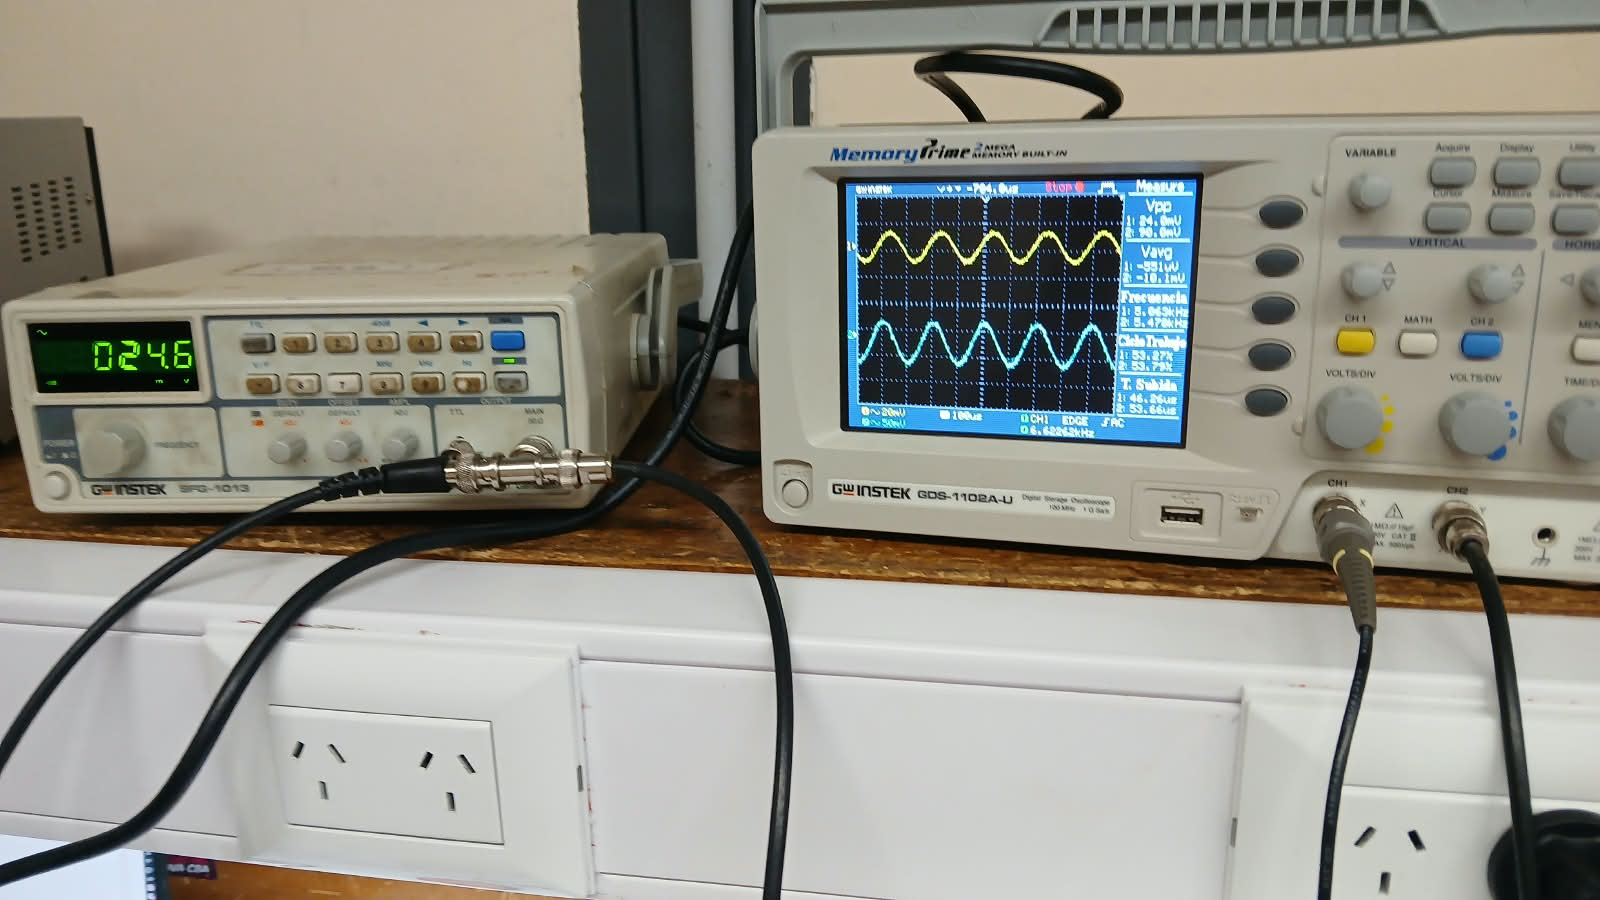
\includegraphics[width=0.8\textwidth]{FotosMed/Impedancias/ZINTOTALSOCLO.jpeg}
    \caption{Pantalla del Osciloscopio}
    \label{fig:osciloscopioZin}
\end{figure}

En \ref{fig:osciloscopioZin} se observa como se utilizaron los instrumentos.

\subsection{Voltaje Máximo de funcionamiento}
Se utilizo la misma configuracion de medicion que en el caso del Barrido de Frecuencia, se mostrara como ejemplo el soporte maximo de tension del circuito total. 

\begin{figure}[H]
    \centering
    % Primera minipage (ocupa el 45% del ancho de la página)
    \begin{minipage}{0.45\textwidth}
        \centering
        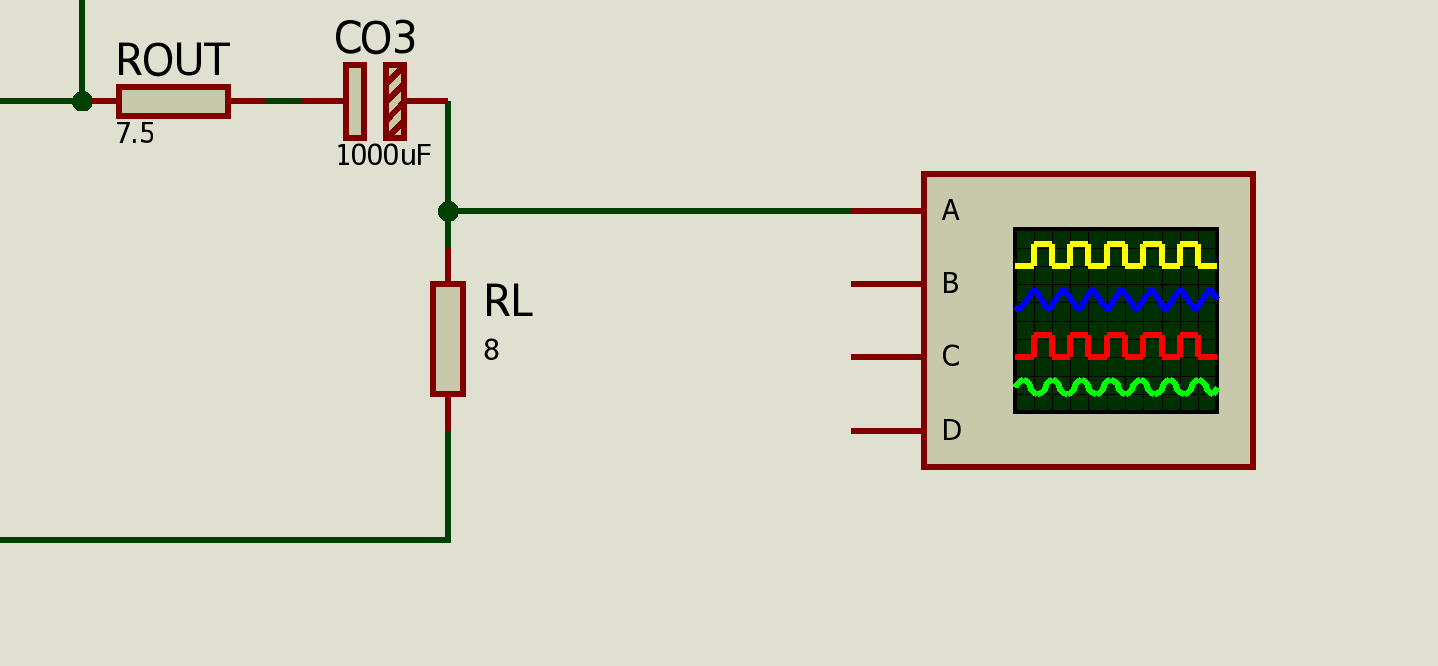
\includegraphics[width=\textwidth]{SetupMediciones/TensionesCorrientes/MaxTension.png} % Ajusta el ancho al de la minipage
        \caption{Representacion esquematica.}
        \label{fig:esquematicpMaxTension}
    \end{minipage}
    \hfill % Relleno elástico para separar las imágenes
    % Segunda minipage (ocupa el 45% del ancho de la página)
    \begin{minipage}{0.45\textwidth}
        \centering
        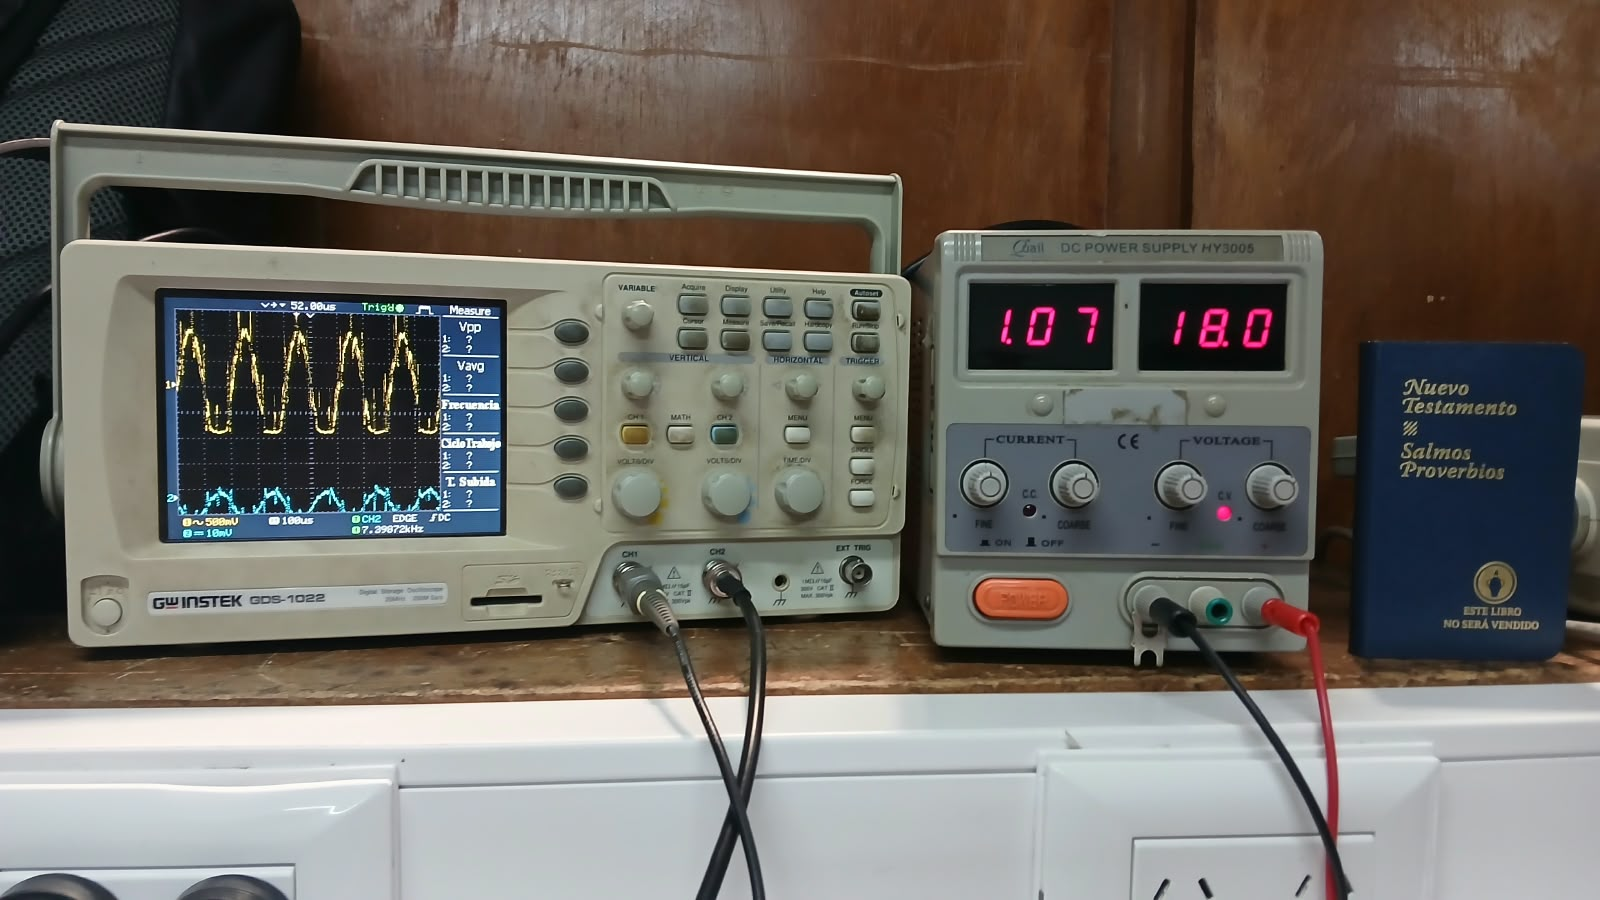
\includegraphics[width=\textwidth]{FotosMed/Voltajesycargademuerte/ARRIBAE123(1).jpeg}
        \caption{Imagen de la Medicion.}
        \label{fig:medicionMAxTension}
    \end{minipage}
\end{figure}

Los 18V en \ref{fig:medicionMAxTension} muestran el voltaje maximo que soporta el circuito, la particularidad de esta medición es que es la tension maxima que soporta el Sziklai, por lo que la maxima tension total esta limitada por la maxima de la última etapa.

\subsection{Voltaje Minimo de funcionamiento}
 Ahora, y con la misma configuracion que la medición anterior, se fue variando la amplitud de la fuente variable y observando la salida por el osciloscopio, el criterio de falla fue no cumplir con el requsito de ganancia. 

 Se usa de ejemplo el circuito total.

\begin{figure}[H]
    \centering
    % Primera minipage (ocupa el 45% del ancho de la página)
    \begin{minipage}{0.45\textwidth}
        \centering
        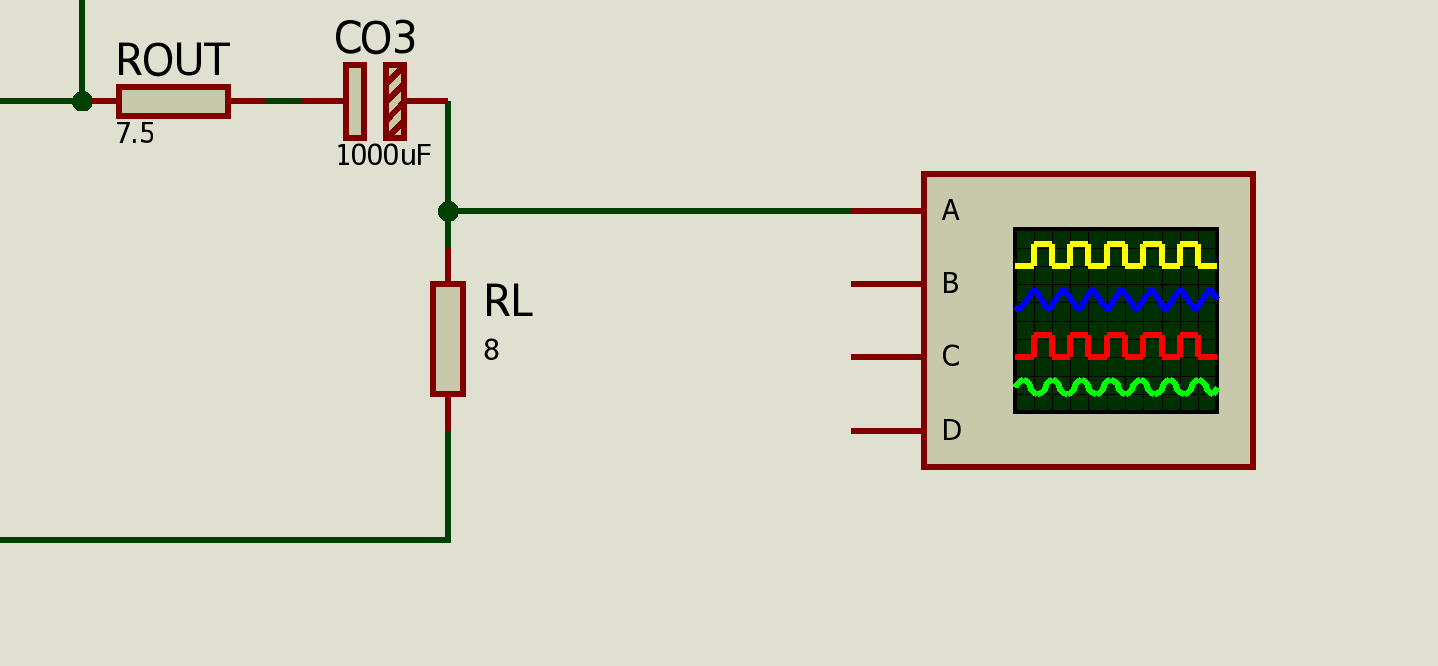
\includegraphics[width=\textwidth]{SetupMediciones/TensionesCorrientes/MaxTension.png} % Ajusta el ancho al de la minipage
        \caption{Representacion esquematica.}
        \label{fig:esquematicpVminimo}
    \end{minipage}
    \hfill % Relleno elástico para separar las imágenes
    % Segunda minipage (ocupa el 45% del ancho de la página)
    \begin{minipage}{0.45\textwidth}
        \centering
        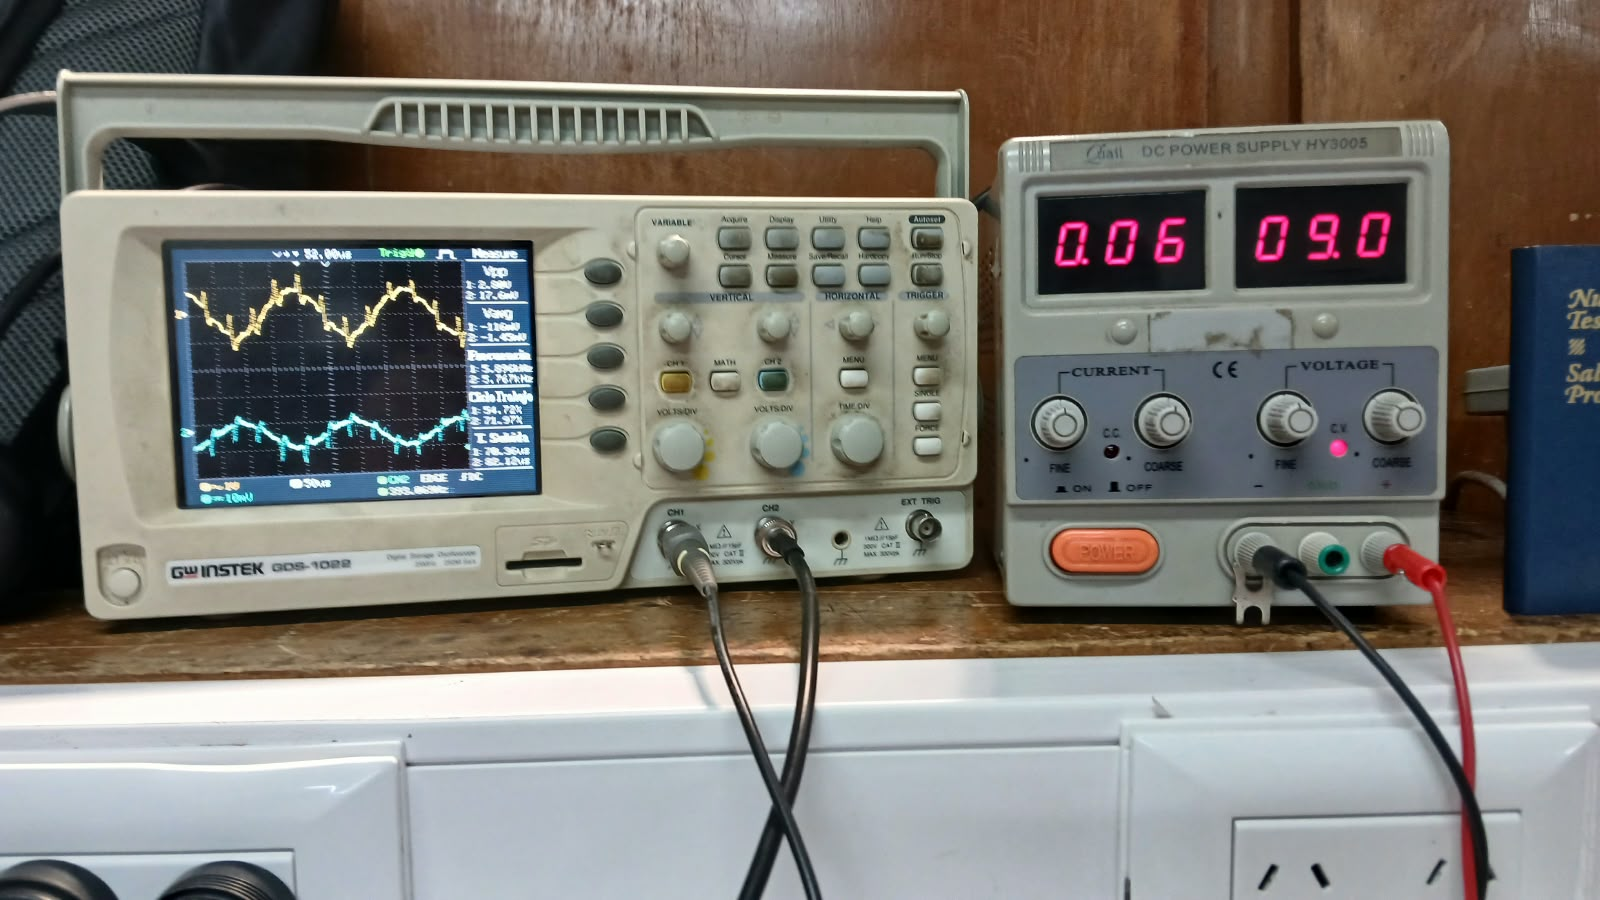
\includegraphics[width=\textwidth]{FotosMed/Voltajesycargademuerte/ABAJOE123(1).jpeg}
        \caption{Imagen de la Medicion.}
        \label{fig:medicionVminimo}
    \end{minipage}
\end{figure}

En \ref{fig:medicionVminimo} se presenta un caso similar a la tensión máxima, el valor de la tensión mínima de funcionamiento esta dado por el valor mínimo de funcionamiento de una de las etapas, en este caso, del emisor común.

\subsection{Resistencia minima de funcionamiento}
Con una configuración parecida a los anteriores, se fueron conectando resistencias en paralelo a la Rl hasta encontrar la resistencias en donde la ganancio no cumple la consigna.

\begin{figure}[H]
    \centering
    % Primera minipage (ocupa el 45% del ancho de la página)
    \begin{minipage}{0.45\textwidth}
        \centering
        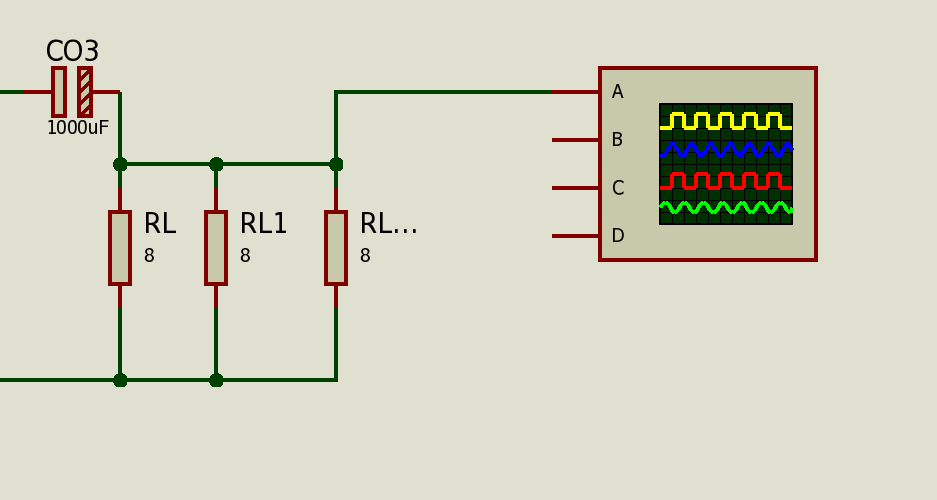
\includegraphics[width=\textwidth]{SetupMediciones/TensionesCorrientes/RdeCorte.png} % Ajusta el ancho al de la minipage
        \caption{Representacion esquematica.}
        \label{fig:esquematicoRCorte}
    \end{minipage}
    \hfill % Relleno elástico para separar las imágenes
    % Segunda minipage (ocupa el 45% del ancho de la página)
    \begin{minipage}{0.45\textwidth}
        \centering
        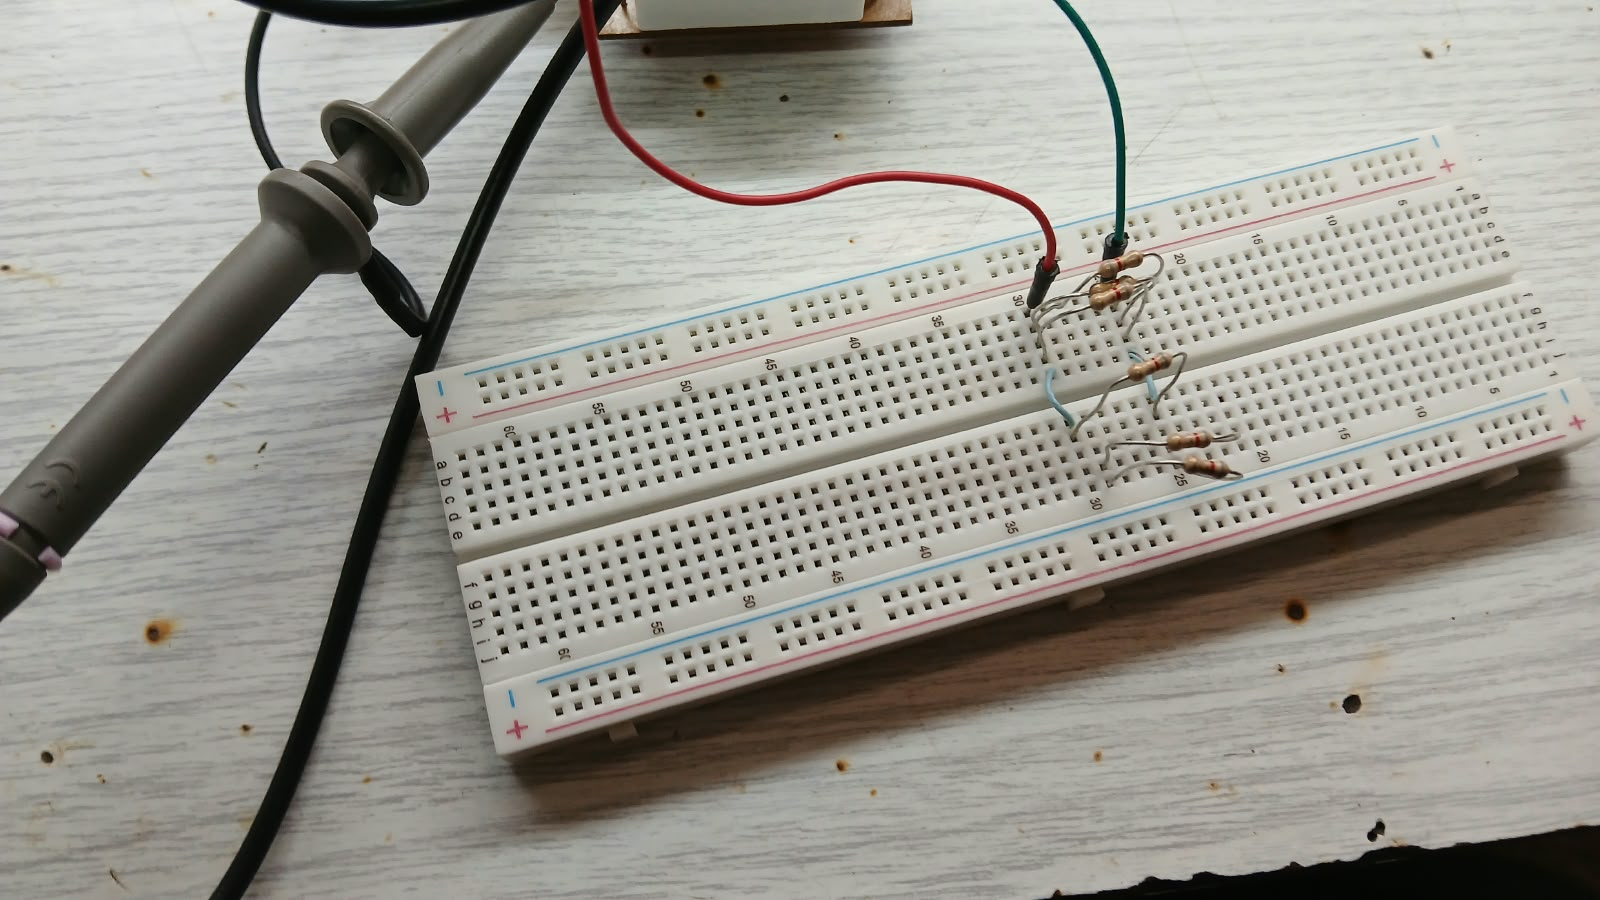
\includegraphics[width=\textwidth]{FotosMed/Voltajesycargademuerte/RMUERTE.jpeg}
        \caption{Imagen de la Medicion.}
        \label{fig:medicionRMuerte}
    \end{minipage}
\end{figure}

\begin{figure}[H]
    \centering
    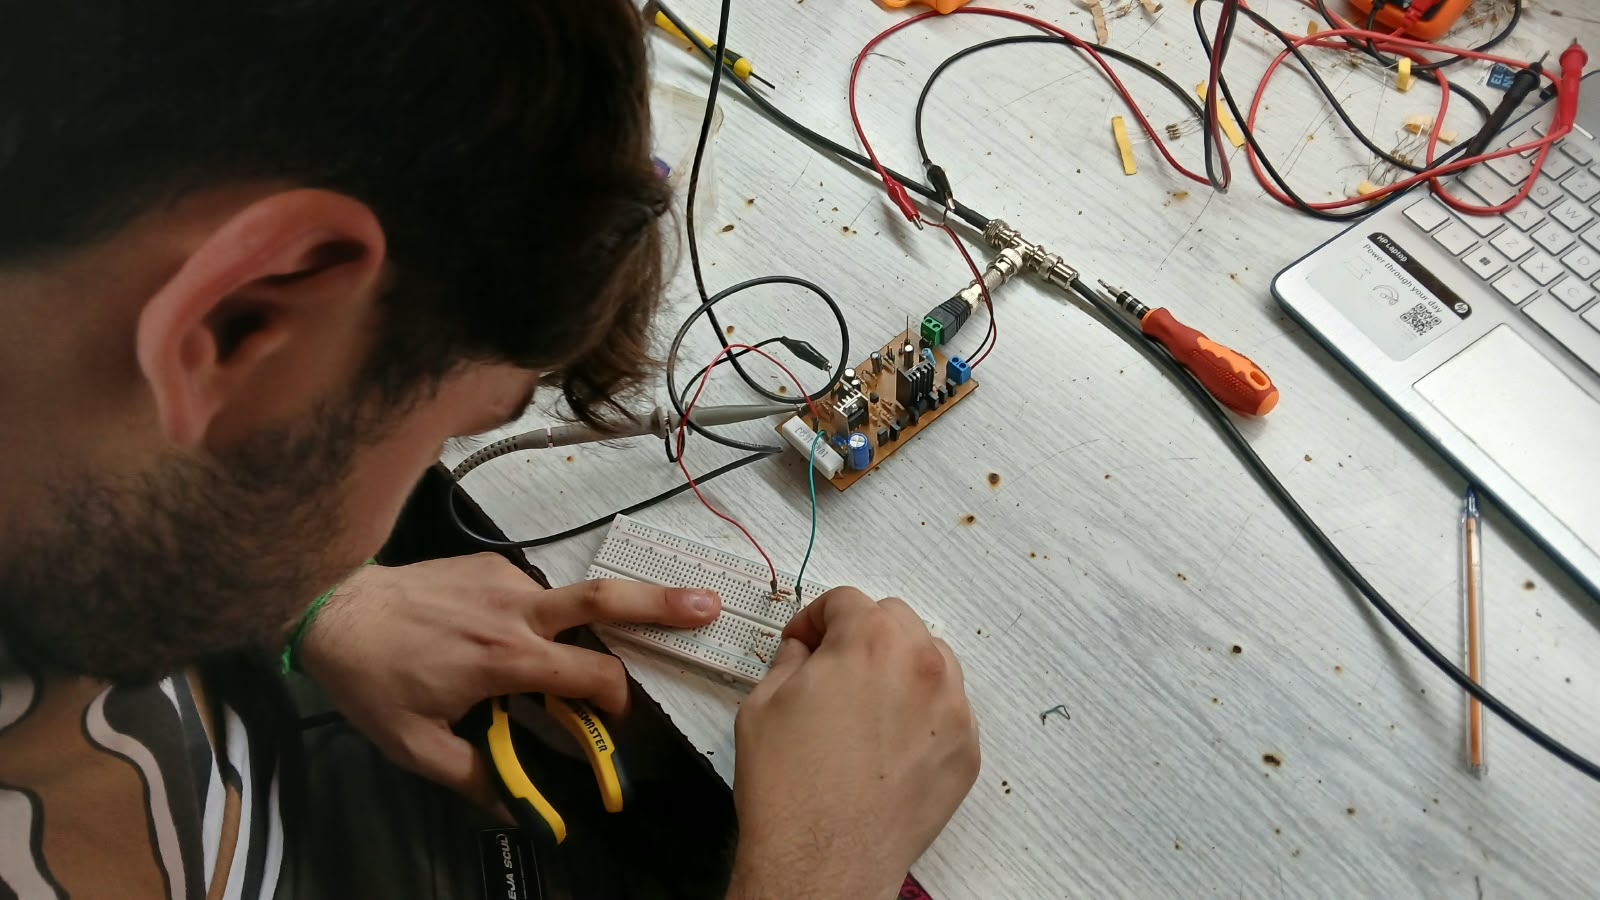
\includegraphics[width=0.8\textwidth]{FotosMed/Voltajesycargademuerte/BuenHombreExplotado.jpeg}
    \caption{Pantalla del Osciloscopio}
    \label{fig:BuenHombreExplotado}
\end{figure}

Se observa en \ref{fig:medicionRMuerte} la disposición de las resistencias de 8.2 Ohm en paralelo, se fueron agregando hasta fallar el requisito de ganancia.
